\chapter{Stopping Criterion for Randomized Low-Rank Approximations}
\label{chap:random}
\epigraph{The probability professor points to a random student
    in the third row and says ``Get out. I do not teach unlucky students.''}{
    One way to start a probablity course; suggested by Elliot Hudgins}

There has been work in recent years to understand
structured matrices: matrices with off-diagonal blocks that
are (or can be approximated as) low-rank.
The goal is to develop methods which allow us to compute
matrix-vector products and matrix inverses faster than
standard algorithms; that is, multiplication in $O(n\log^{\beta}n)$
flops and inversion in $O(n^{\alpha}\log^{\beta}n)$ flops
for $\alpha\in\brackets{1,2}$ and $\beta$ small.
Another benefit is reduced storage requirements,
frequently $O(n\log^{\beta}n)$.
The simplest of these are banded matrices, but also include
Sequentially Semi-Separable matrices~\cite{chandrasekaran2005some},
Hierarchically Semi-Separable (HSS)
matrices~\cite{Chandrasekaran2005HSS,chandrasekaran2006fast},
H-matrices~\cite{hackbusch1999sparse}, and others.
Recent work involving randomized HSS construction can be found in
\cite{martinsson2011fast,rouet2016distributed,ghysels2017robust}.
The main contribution of this chapter is related to
a stochastic estimate of $\norm{\cdot}_{F}$ which
allows us to accurately measure the low-rank approximation
and determine when it is well-approximated;
portions of this material first appeared in~\cite{randomHSSLBL}.
In particular, we develop a method to compute a \emph{relative}
stopping criterion for an adaptive low-rank approximation.

Throughout this chapter we assume $A\in\R^{m\times n}$
with rank $r\ll \min(m,n)$.
For simplicity, we will assume $m\ge n$.
We let $N(0,1)$ refer to the standard normal distribution
with mean $0$ and variance $1$.
Finally, some of the notation in this chapter may conflict with those
from previous chapters.
While other adaptive randomized algorithms have frequently used
an absolute tolerance $\eps$, we will focus on allowing both
an absolute tolerance $\epsa$ and a relative tolerance $\epsr$.

% Section: Randomized Low-Rank Approximation
% Label: \ref{sec:rand_lra}
\section{Randomized Low-Rank Approximation}
\label{sec:rand_lra}

In recent years there has been growing interest in using randomization
to speed up conventional numerical linear algebra techniques;
one standard reference is~\cite{RandomReview2011}.
The main idea is that we would like to compute
accurate factorizations like pivoted QR or the SVD on low-rank matrices.
These factorizations usually have  flop counts of
$O(mnr)$ and $O(mn^{2})$, respectively,
but the data transfer required makes these computations expensive,
especially when matrices are so large as to not fit in fast memory.
Thus, it is impractical to use standard dense algorithms with
large communication costs on distributed memory machines.
By looking at random samplings of the range, the desire is
to build up an approximation of the matrix until reaching
a predetermined approximation tolerance.
Once a sufficient number of random samples have been computed,
we perform a pivoted QR or SVD on this smaller dense
matrix, leading to a smaller overall cost.
The random samplings are computed using matrix-matrix multiplication,
which can be efficiently computed on modern hardware.
Although these multiplications may be a significant portion
of the overall flop count, the total time
spent performing multiplication is small.
Thus, the goal is to determine when enough samples have been computed
to ensure an accurate approximation of the matrix.
The standard algorithm for building a low-rank approximation
is found in Alg.~\ref{alg:rand_low_rank}, with the primary
arguments being the block size $d$ and \texttt{stopping\_criterion},
a function which determines when we have a good enough approximation
of the range of $A$; similar blocked algorithms can be found
in~\cite{yu2018efficient,martinsson2016randomized} and are reproduced below.
In Line~\ref{alg_line:rand_Gen_GS} of Alg.~\ref{alg:rand_low_rank},
we perform iterated Gram-Schmidt orthogonalization for numerical stability,
as it helps ensure $Q$ is \emph{numerically} orthogonal to machine
precision, especially in the blocked case~\cite{bjorck1994GS,stewart2008}.
This may not always be necessary, for \cite{stewart2008} notes
this would only be required should the column norms decrease by a significant
factor; even so, algorithmically it is easier, though more expensive,
to always perform iterated GS.
Additionally, although \texttt{rand} could produce any kind of random
matrices, our analysis requires us to use Gaussian random variables.
See Table~\ref{tab:rand_helper_funcs} for a list of helper functions
for the algorithms in this chapter.
We denote the pivoted QR factorization as \texttt{rrqr}
and it stops when $\abs{R_{k,k}}<\epsa$ or
$\abs{R_{k,k}} < \epsr\abs{R_{1,1}}$.

\begin{table}
\centering
\begin{tabular}{r|p{0.7\textwidth}}
\hline
\texttt{rand}(m,n) & an $m\times n$ matrix with iid $N(0,1)$ elements \\
\texttt{cols}(A) & number of columns of $A$ \\
$\texttt{qr}(A)$ & unpivoted QR factorization of $A$ returning $Q$
    or $Q$ and $R$ \\
$\texttt{rrqr}(A,\epsa,\epsr)$ & rank-revealing QR factorization of $A$
    such as QRCP with absolute/relative tolerances $\epsa$/$\epsr$ \\
\hline
\end{tabular}
\caption[List of helper functions for low-rank approximation]{
List of helper functions for low-rank approximation.}
\label{tab:rand_helper_funcs}
\end{table}


These algorithms frequently use a QB approximation of $A$.
Here $Q$ is an approximate orthonormal basis for the range of $A$
with $B = Q^{*}A$; that is
%
\begin{align}
    A &\approx Q(Q^{*}A) \nonumber\\
    &= QB.
\end{align}
%
Knowing when $\norm{A - QB}$ is small is our primary concern,
and the particular choice of norm is important.
This chapter will investigate when this happens,
propose a new method, and compare it with existing stopping criteria.
The stopping criterion presented here has focused on developing
a \emph{relative} stopping criterion.
This is particularly useful as it may be more convenient
to specify a relative error tolerance over an absolute tolerance.
Furthermore, we would like this method to work in the case
we do not have explicit access to the matrix.
Theorem 4.2 in~\cite{vogel2016superfast} says that if $H$ is a
structured $N\times N$ matrix and $\widetilde{H}$ is $H$
with off-diagonal blocks truncated
to tolerance $\epsr$, then
%
\begin{equation}
    ||H - \widetilde{H}||_{F} \le C(N,L)\epsr\norm{H}_{F}.
\end{equation}
%
Thus, it makes sense to seek an accurate relative stopping criterion.
Once a sufficient number of random samples have been computed,
we perform a pivoted QR factorization
(such as QR with Column Pivoting, although the Strong RRQR
from~\cite{gu1996efficient} would be better) on these samples
in order to obtain a high-quality $Q$ for a better QB approximation.
While this last step may not be necessary and was not included
in~\cite{yu2018efficient,martinsson2016randomized},
this would be an easy step to add and was desired in
the original setting where this stopping criterion was
developed~\cite{randomHSSLBL}.

\begin{algorithm}[t]
\caption{Randomized Block Low-Rank Approximation (General)}
\label{alg:rand_low_rank}
\begin{algorithmic}[1]
\Function{random\_low\_rank}{$A$,$d$,\texttt{stopping\_criterion}}
\Comment{Builds $QB$ approximation}
    \State $Q = [\,]$; $n = \texttt{cols}(A)$
    \State $k=0$
    \While {!\texttt{stopping\_criterion}($Q$,$A$,$\eps$)}
        \State $k = k + 1$
        \State $\Omega_{k} = \texttt{rand}(n,d)$
        \Comment{$d$ is block size}
        \State $S_{k} = A\Omega_{k}$
        \State $\widehat{S}_{k} = \parens{I - QQ^{*}}^{2}S_{k}$
        \Comment{$2\times$ GS orthogonalization for numerical stability}
        \label{alg_line:rand_Gen_GS}
        \State $[Q_{k},R_{k}] = \texttt{qr}(\widehat{S}_{k})$
        \State $Q = \begin{bmatrix}Q & Q_{k}\end{bmatrix}$
    \EndWhile
\State $B = Q^{*}A$
\State \Return $Q$, $B$
\Comment{We have the approximation $A \approx QB$}
\EndFunction
\end{algorithmic}
\end{algorithm}


We recall the Eckhart-Young theorem~\cite[Theorem~1.1]{gu2015subspace},
which gives optimal low-rank approximation bounds in the 2-norm and F-norm:

\begin{thm}[Eckhart-Young Theorem]
If $A_{k}$ is the matrix $A$ chopped to $k$ singular values,
then we have the following bounds on approximations of $A$:
%
\begin{align}
    \min_{\text{rank}(B)\le k}\norm{A-B}_{2} &= \norm{A-A_{k}}_{2} \nonumber\\
        &= \sigma_{k+1} \nonumber\\
    \min_{\text{rank}(B)\le k}\norm{A-B}_{F} &= \norm{A-A_{k}}_{F} \nonumber\\
        &= \sqrt{\sum_{j=k+1}^{\min(m,n)}\sigma_{j}^{2}}.
\end{align}
\end{thm}

\noindent
In practice, we hope to be able to determine approximations
with near-optimal ranks within a specified tolerance
with smaller overall computation time.
Thus, we are looking at the fixed-precision low-rank approximation problem.




\section{Stopping Criteria}
\label{sec:rand_stop_crit}

The unitary invariance of the 2-norm combined with it being
the definition of the operator (matrix) norm makes it
desirable to bound $\norm{(I-QQ^{*})A}_{2}$.
The main challenge of the 2-norm stems from the computational
complexity required to compute it exactly.
Because of this, the F-norm is the next norm that we may wish
to bound, and it is easy to compute if we have explicit access to the matrix
in question; furthermore, it trivially bounds the 2-norm.
If $A$ is large or implicitly defined, $\norm{A}_{F}$ may still be expensive
to compute.
Additionally, the exact norm is frequently not required so much as
an accurate approximation of it.
We will be making comparisons with algorithms
in~\cite{martinsson2016randomized,yu2018efficient}, so we reproduce
their blocked versions here.
Alg.~\ref{alg:rand_low_rank_MV}
is from~\cite[Figure 2]{martinsson2016randomized} (the MV Algorithm,
named after the authors)
and Alg.~\ref{alg:rand_low_rank_YGL}
is from~\cite[Algorithm 2]{yu2018efficient} (the YGL Algorithm,
named after the authors).
Algs.~\ref{alg:rand_low_rank_MV} and \ref{alg:rand_low_rank_YGL} originally
used $Q = \texttt{orth}(A)$ to compute the orthonormal basis
of a matrix $A$; this work uses the function \texttt{qr} in our notation
because it is an unpivoted QR factorization,
and our new stopping criterion will require both $Q$ and $R$ factors
of the unpivoted QR factorization.
A variation of iterated Gram-Schmidt orthogonalization can be found in
Line~\ref{alg_line:rand_MV_GS}  of Alg.~\ref{alg:rand_low_rank_MV}  and
Line~\ref{alg_line:rand_YGL_GS} of Alg.~\ref{alg:rand_low_rank_YGL}
to help $Q$ retaining numerical orthogonality.
It is explicitly stated in~\cite[Remark 5]{martinsson2016randomized}
that the fact $R$ is not used in the \texttt{qr} routine
(original \texttt{orth}).
From our work here, we see the $R$ factor helps ensure we do
not take too many random samples by noting when the $R$-values become small.
Even so, no pivoting is required.


\begin{algorithm}[p]
\caption{Randomized Block Low-Rank Approximation (MV)
    \cite[Figure 2]{martinsson2016randomized}}
\label{alg:rand_low_rank_MV}
\begin{algorithmic}[1]
\Function{randQB\_b\_MV}{$A$,$\eps$,$d$}
    \For {$k=1,2,3,\cdots$}
        \State $\Omega_{k} = \texttt{rand}(n,d)$
        \State $Q_{k} = \texttt{qr}(A\Omega_{k})$
        \State $Q_{k} = \texttt{qr}(Q_{k}-\sum_{j=1}^{k-1}Q_{j}Q_{j}^{*}Q_{k})$
            \label{alg_line:rand_MV_GS}
        \State $B_{k} = Q_{k}^{*}A$
        \State $A = A - Q_{k}B_{k}$
        \If {$\norm{A} < \eps$}
            \State \textbf{stop}
        \EndIf
    \EndFor
\State $Q = \begin{bmatrix} Q_{1} & \cdots & Q_{k} \end{bmatrix}$
\State $B = \begin{bmatrix} B_{1}^{*} & \cdots & B_{k}^{*} \end{bmatrix}^{*}$
\State \Return $Q$, $B$
\EndFunction
\end{algorithmic}
\end{algorithm}

\begin{algorithm}[p]
\caption{Randomized Block Low-Rank Approximation (YGL)
    \cite[Algorithm 2]{yu2018efficient}}
\label{alg:rand_low_rank_YGL}
\begin{algorithmic}[1]
\Function{randQB\_b\_YGL}{$A$,$\eps$,$d$}
\State $Q = [\,]$; $B = [\,]$
\State $E = \norm{A}_{F}^{2}$
    \For {$k=1,2,3,\cdots$}
        \State $\Omega_{k} = \texttt{rand}(n,d)$
        \State $Q_{k} = \texttt{qr}(A\Omega_{k} - Q(B\Omega_{k}))$
        \State $Q_{k} = \texttt{qr}(Q_{k} -Q (Q^{*}Q_{k}))$
            \label{alg_line:rand_YGL_GS}
        \State $B_{k} = Q_{k}^{*}A$
        \State $Q = \begin{bmatrix} Q & Q_{k} \end{bmatrix}$
        \State $B = \begin{bmatrix} B^{*} & B_{k}^{*} \end{bmatrix}^{*}$
        \State $E = E - \norm{B_{k}}_{F}^{2}$
        \If {$E < \eps^{2}$}
            \State \textbf{stop}
        \EndIf
    \EndFor
\State \Return $Q$, $B$
\EndFunction
\end{algorithmic}
\end{algorithm}


One stopping criterion is based on the following lemma~\cite{RandomReview2011}:

\begin{lem}[HMT Error Bound;
    Lemma 4.1 in~\cite{RandomReview2011}]
\label{thm:rand_hmt_bound}
Let $B\in\R^{m\times n}$. Fix a positive integer $d$ and $\alpha>1$.
Draw an independent family of standard Gaussian vectors
$\braces{\omega_{k}}_{k=1}^{d}$.
Then
%
\begin{equation}
    \norm{B}_{2} \le \alpha\sqrt{\frac{2}{\pi}}\max_{k=1,\cdots,d}
        \norm{B\omega_{k}}_{2}
    \label{eq:rand_hmt_bound}
\end{equation}
%
with probability $1-\alpha^{-d}$.
\end{lem}

\noindent
The reference to ``HMT'' comes from the first letters of
the authors' last names in~\cite{RandomReview2011}
and is used in~\cite[Alg.~4.2]{RandomReview2011}
(Adaptive Randomized Range Finder).
Here, $\alpha$ can be viewed as a trade-off parameter: larger values
ensure a smaller probability of failure.
It turns out, though, this overestimation is significant; this will
be shown for a number of matrices in Sec.~\ref{sec:rand_exp}.
We can find no references to randomized lower bounds of $\norm{B}_{2}$;
this would be helpful in producing an order-of-magnitude estimate
or estimates relating to the variance or other moments of the random variable.
This method is used in~\cite{liu2016parallel,xi2014fast,saibaba2016randomized}
as a stopping criterion for adaptive randomized algorithms
for structured matrices
(the same situation where this work was originally developed).

The authors in \cite{martinsson2016randomized} note the drawback of
Lem.~\ref{thm:rand_hmt_bound} of this over estimation and instead
use the explicit bound $\norm{A}<\eps$ in Alg.~\ref{alg:rand_low_rank_MV},
where we note $A$ is updated every time after having known
information subtracted out during each iteration.
The authors said that $\norm{A}_{2}$ could be used but noted
that $\norm{A}_{F}$ may be preferred for its easy computation.
One drawback (noted in~\cite{yu2018efficient}) is that this requires 
access to a dense copy of $A$.
This is problematic with regards to memory because we may
want to keep an unmodified version of the original matrix; furthermore,
if $A$ is originally sparse, it will immediately become dense
after subtracting the first approximation,
greatly increasing memory requirements.

This resulted in the development of the stopping criterion
in~\cite{yu2018efficient}.
Instead of storing a dense matrix with the unused information
of $A$ to keep track of the error, it is possible to compute
the error just based on the difference in F-norm.
This is made explicit in the next theorem, which we call
the ``YGL Error Bound'' because of the first letters
of the authors' last names.
Calling this an error bound is slightly misleading because the
error is exact, not bounded, but a better title escapes us at this time.

\begin{thm}[YGL Error Bound;
    Theorem 1.1 in~\cite{yu2018efficient}]
\label{thm:rand_ygl_bound}
Let $A\in\R^{m\times n}$ and $Q\in\R^{n\times k}$ be orthogonal.
If $B = Q^{*}A$ then
%
\begin{equation}
    \norm{A - QB}_{F}^{2} = \norm{A}_{F}^{2} - \norm{B}_{F}^{2}.
    \label{eq:rand_ygl_bound}
\end{equation}
\end{thm}

\noindent
If one builds up $Q$ in blocks, then we can compute the true F-norm error
provided $\norm{A}_{F}$ is already known.
Because this value only needs to be computed once, it may not 
be too expensive;
however, this only works if the matrix is explicitly, not implicitly, defined.
Additionally, Thm.~\ref{thm:rand_ygl_bound} is only useful
for relative tolerances down to $O(\sqrt{\epsm})$,
where $\epsm$ is machine precision,
as noted in~\cite[Theorem 3]{yu2018efficient}.
It is possible, using techniques such as compensated
summation~\cite[Chapter 4]{HighamASNA}, that these limitations may be
lifted, but this would be difficult in the parallel setting.
This may be the first explicit reference to a relative error bound
in the literature, though we seek to remove the relative tolerance restrictions.



\section{Previous Probabilistic Bounds}

We now present results from~\cite{gu2015subspace}, although
looser bounds from~\cite{RandomReview2011} may be more well-known.
The important portions of the bounds will be emphasized here;
the original paper should be referenced for the full results and proofs.

\begin{thm}[Average 2-Norm and F-Norm Error;
    Theorem 5.7 in~\cite{gu2015subspace}]
\label{thm:rand_ave_2_F_norm_err_gu}
Let $\Omega$ be a Gaussian random matrix with $k+p$ columns for
$p\ge2$, $S = (AA^{*})^{q}A\Omega$, and $Q = \texttt{qr}(S)$.
Then
%
\begin{align}
    \E\norm{A-QQ^{*}A}_{2} &\le
        \sqrt{\sigma_{k+1}^{2} + C(A,k,p,q)} \nonumber\\
    \E\norm{A-QQ^{*}A}_{F} &\le
        \sqrt{\parens{\sum_{j=k+1}^{n}\sigma_{j}^{2}} + D(A,k,p,q)}
\end{align}
%
Here, $C$ and $D$ are constants which decay exponentially as $q$ increases.
\end{thm}

\noindent
The above theorem states the expected value of the error is close to optimal.
Similar results hold for upper tail bounds:

\begin{thm}[Probability Tail Bounds in 2-Norm and F-Norm;
    Theorem 5.8 in~\cite{gu2015subspace}]
Let the assumptions of Thm.~\ref{thm:rand_ave_2_F_norm_err_gu} hold.
Then if $0<\Delta\ll1$,
%
\begin{align}
    \norm{A-QQ^{*}A}_{2} &\le
        \sqrt{\sigma_{k+1}^{2} + C(A,k,p,q,\Delta)} \nonumber\\
    \norm{A-QQ^{*}A}_{F} &\le
        \sqrt{\parens{\sum_{j=k+1}^{n}\sigma_{j}^{2}} + D(A,k,p,q,\Delta)}
\end{align}
%
hold for probability $1-\Delta$.
$C$ and $D$ are constants which decay exponentially as $q$ increases.
\end{thm}

\noindent
Additionally, \cite[Theorem 5.6]{gu2015subspace} bounds deviations
of the singular values of $QQ^{*}A$ from the singular values of $A$.

These are useful results and help explain why randomized methods
perform better than expected if one looks at similar
bounds in~\cite{RandomReview2011}.
The downside is that in practice they are not helpful because
we must know the singular values.

In these theorems, $q$ refers to the possibility of using
power iteration in order to increase the quality of the approximation;
this is a well-known technique in randomized numerical linear
algebra~\cite{RandomReview2011,yu2018efficient,
martinsson2016randomized} and helps ensure the larger singular values
and corresponding singular vectors are matched more
closely~\cite{gu2015subspace,saibaba2019randomized}.
Power iteration is not mentioned in~\cite{randomHSSLBL}
because it is not clear how to use it in
randomized HSS construction without greatly increasing the
overall computational cost; it is likely this also holds in general
for the randomized construction of structured matrices
because we do not have explicit access to matrix subblocks.
This lead to the desire for an accurate method to determine
low-rank approximations which could be used with small relative
tolerances (for example, tolerances as small as
$10^{-5}$ in single precision and $10^{-14}$ in double precision).


\section{Basic Probability Theory}
\label{sec:rand_prob_theory_intro}

We assume $A$ has positive singular values
$\sigma_{1}\ge\cdots\ge\sigma_{r}>0$.
It follows that we have the SVD
%
\begin{align}
    A &= U\Sigma V^{*} \nonumber\\
    &= \begin{bmatrix} U_{1} & U_{2} \end{bmatrix}
        \begin{bmatrix} \Sigma_{r} & 0 \\ 0 & 0 \end{bmatrix}
        \begin{bmatrix} V_{1}^{*} \\ V_{2}^{*} \end{bmatrix} \nonumber\\
    &= U_{1}\Sigma_{r}V_{1}^{*},
\end{align}
%
where
%
\begin{equation}
    \Sigma_{r} = \diag\parens{\sigma_{1},\cdots,\sigma_{r}}.
\end{equation}
%
If $x\in\R^{n}$ is a Gaussian random vector (that is, $x_{i}\sim N(0,1)$)
and we set $\xi = V^{*}x$, then by the rotational invariance
of $\norm{\cdot}_{2}$ we have
%
\begin{align}
    \norm{Ax}_{2}^{2} &= \norm{\Sigma_{r}\xi}_{2}^{2} \nonumber\\
        &= \sigma_{1}^{2}\xi_{1}^{2} + \cdots + \sigma_{r}^{2}\xi_{r}^{2}.
\end{align}
%
Now, $\xi_{i}\sim N(0,1)$ because rotations of Gaussian random vectors
are also Gaussian random vectors.
From here, we can see
%
\begin{equation}
    \E\norm{Ax}_{2}^{2} = \norm{A}_{F}^{2}.
\end{equation}
%
This by itself is useful, but, in order to make use of
computer architecture, matrix-matrix products are preferred over
multiple matrix-vector products.
Thus, if $\Omega\in\R^{n\times d}$ with $\Omega_{ij}\sim N(0,1)$
(so that $\Omega$ is a Gaussian random matrix), it follows that
%
\begin{equation}
    \norm{A\Omega}_{F}^{2} = \norm{A\Omega_{:,1}}_{2}^{2} + \cdots
        + \norm{A\Omega_{:,d}}_{2}^{2}.
\end{equation}
%
Because each $\Omega_{:,i}$ is a Gaussian random vector, we also have
%
\begin{equation}
    \E\norm{A\Omega}_{F}^{2} = d\norm{A}_{F}^{2}.
    \label{eq:rand_new_error_bound}
\end{equation}
%
It is this equality that allows us to accurately compute the F-norm
of matrices using random range samples.

Because there is interest in using power iterations to increase
the quality of randomized low-rank factorizations~\cite{RandomReview2011},
we also include these related results.
In particular, it is clear from the previous work that
%
\begin{align}
    \norm{\parens{AA^{*}}^{q}Ax}_{2}^{2}
        &= \sigma_{1}^{4q+2}\xi_{1}^{2} + \cdots + \sigma_{r}^{4q+2}\xi_{r}^{2}
        \nonumber\\
    \norm{\parens{A^{*}A}^{q}x}_{2}^{2}
        &= \sigma_{1}^{4q}\xi_{1}^{2} + \cdots + \sigma_{r}^{4q}\xi_{r}^{2},
\end{align}
%
so we have
%
\begin{align}
    \E\norm{\parens{AA^{*}}^{q}Ax}_{2}^{2}
        &= \norm{A}_{s,4q+2}^{4q+2}
        \nonumber\\
    \E\norm{\parens{A^{*}A}^{q}x}_{2}^{2}
        &= \norm{A}_{s,4q}^{4q}
\end{align}
%
and
%
\begin{align}
    \E\norm{\parens{AA^{*}}^{q}A\Omega}_{2}^{2}
        &= d\norm{A}_{s,4q+2}^{4q+2}
        \nonumber\\
    \E\norm{\parens{A^{*}A}^{q}\Omega}_{2}^{2}
        &= d\norm{A}_{s,4q}^{4q}.
    \label{eq:rand_new_power_error_bound}
\end{align}
%
Here, $\norm{\cdot}_{s,p}$ is the Schatten $p$-norm defined
in Eq.~\eqref{eq:kar_schatten_def} and $\Omega$ is a Gaussian random
matrix with $d$ columns, as before.
From the definitions of the Schatten $p$-norm, it is clear
%
\begin{align}
    \brackets{\E\norm{\parens{AA^{*}}^{q}Ax}_{2}^{2}}^{1/4q+2}
        &\to \norm{A}_{2}
        \nonumber\\
    \brackets{\E\norm{\parens{A^{*}A}^{q}x}_{2}^{2}}^{1/4q}
        &\to \norm{A}_{2}
        \nonumber\\
    \brackets{\E\norm{\parens{AA^{*}}^{q}A\Omega}_{2}^{2}}^{1/4q+2}
        &\to \norm{A}_{2}
        \nonumber\\
    \brackets{\E\norm{\parens{A^{*}A}^{q}\Omega}_{2}^{2}}^{1/4q}
        &\to \norm{A}_{2}
\end{align}
%
as $q\to\infty$.

The proof that independent realizations of Eqs.~\eqref{eq:rand_new_error_bound}
and \eqref{eq:rand_new_power_error_bound}
produce accurate approximations of the F-norm and Schatten norm
will be postponed until Sec.~\ref{sec:rand_prob_theory_proofs}.
We now focus on developing our stopping criterion, which is based on
the fact that we can now accurately estimate our error in a matrix norm.





\section{New Stopping Criterion}
\label{sec:rand_new_stopping}

We now step through Alg.~\ref{alg:rand_low_rank} to see
where some problems, previously ignored, may arise;
this stems from the fact that we are wanting to be able to have
relative error tolerances on the order of $10^{-12}$ or $10^{-14}$
in double precision.
We will be building our random matrices up in blocks of $d$ random
vectors at a time, although in theory the size of the blocks could vary.
Assume we have our absolute tolerance $\epsa$ and relative tolerance $\epsr$.
Then our \texttt{stopping\_criterion} function will return \texttt{true} if
%
\begin{equation}
    ||\widehat{S}_{k}||_{F} < \max(\epsa\sqrt{d},\epsr\norm{S_{k}}_{F});
\end{equation}
%
otherwise, \texttt{stopping\_criterion} returns \texttt{false}.

\begin{enumerate}

\item Set $\Omega_{i} = \texttt{rand}(n,d)$ and compute $S_{i} = A\Omega_{i}$
for $i\in\braces{1,2}$; set $Q = [\,]$ and
$S = \begin{bmatrix} S_{1} & S_{2} \end{bmatrix}$.

\item Compute $[Q_{1},R_{1}] = \texttt{qr}(S_{1})$,
giving the initial approximation for the range of $A$; set $Q = Q_{1}$.

\item Set $\widehat{S}_{2} = \parens{I-QQ^{*}}^{2}S_{2}$, so that
$\widehat{S}_{2}$ contains potentially new information
about the range of $A$.
If
%
\begin{equation}
    ||\widehat{S}_{2}||_{F} < \max(\epsa\sqrt{d},\epsr||S_{2}||_{F}),
\end{equation}
%
then stop and perform $Q = \texttt{rrqr}(S,\epsa,\epsr)$.

\item Set $\Omega_{3} = \texttt{rand}(n,d)$ and compute $S_{3} = A\Omega_{3}$;
set $S = \begin{bmatrix} S & S_{3} \end{bmatrix}$.

\item Compute $[Q_{2},R_{2}] = \texttt{qr}(\widehat{S}_{2})$,
giving new information for the range of $A$;
set $Q = \begin{bmatrix} Q & Q_{2} \end{bmatrix}$.

\item Set $\widehat{S}_{3} = \parens{I-QQ^{*}}^{2}S_{3}$, so that
$\widehat{S}_{3}$ contains potentially new information
about the range of $A$.
If
%
\begin{equation}
    ||\widehat{S}_{3}||_{F} < \max(\epsa\sqrt{d},\epsr||S_{3}||_{F}),
\end{equation}
%
then stop and perform $Q = \texttt{rrqr}(S,\epsa,\epsr)$.

\item Continue this process until convergence $\dots$

\end{enumerate}

\noindent
Using individual realizations of Eq.~\eqref{eq:rand_new_error_bound}
is important in the stopping criterion, although the relative stopping
$||\widehat{S}_{k}||_{F} < \epsr||S_{k}||_{F}$ is new.
Even so, in order to ensure we are adding new information to $Q$ in steps
2 and 5, we need to know $\widehat{S}_{k}$ is full rank.
This problem does not show up in the unblocked version because
updating $Q$ one vector at a time makes it easy to determine
when a vector has small norm.
This situation, when $\widehat{S}_{k}$ is numerically low-rank,
is not considered in
Algs.~\ref{alg:rand_low_rank_MV} and \ref{alg:rand_low_rank_YGL}
due to how the $Q_{k}$ blocks are formed,
although this is critical to ensure $Q$ has orthonormal columns.
As noted previously, performing multiple matrix-vector multiplications
is inefficient on modern machines, which is why the blocked case is important.
Thus, if $\widehat{S}_{k}$ is (numerically) rank-deficient,
then additional random samples contain no new information above the
specified tolerance and we should
compute the rank-revealing QR factorization on our random samples.
If $\widehat{S}_{k}$ is determined to be rank-deficient, then
$\begin{bmatrix} S_{1} & S_{2} & \cdots & S_{k} \end{bmatrix}$
is rank-deficient.
This implies the random samples matrix
%
\begin{equation}
    S = \begin{bmatrix} S_{1} & S_{2} & \cdots & S_{k} & S_{k+1} \end{bmatrix}.
\end{equation}
%
is rank-deficient as well and the additional block of random samples $S_{k+1}$
should ensure a better quality RRQR factorization than just using
$\begin{bmatrix} S_{1} & S_{2} & \cdots & S_{k} \end{bmatrix}$.
Although this is not a proof, extensive examples
in Sec.~\ref{sec:rand_exp} show that this is expected
and matches our intuition.

To determine numerical rank-deficiency, we set
%
\begin{equation}
    \rho = \frac{||S_{1}||_{F}}{\sqrt{d}},
\end{equation}
%
implying $\rho\approx\norm{A}_{F}$,
and say $\widehat{S}_{k}$ is numerically rank-deficient when
%
\begin{equation}
    \min_{j=1,\cdots,d} |\parens{R_{k}}_{j,j}| < \max(\epsa,\epsr\rho).
\end{equation}
%
The purpose of $\rho$ is to characterize how large the original norms
of the random samples should be, as this will help determine when
they have fallen below the desired tolerance.
Because of this, other potential values of $\rho$ are $|(R_{1})_{1,1}|$,
$\max_{j} |(R_{1})_{j,j}|$, or $\max_{j,k} |(R_{k})_{j,j}|$.
If the desire is to minimize communication, then
$|(R_{1})_{1,1}|$ or $\max_{j} |(R_{1})_{j,j}|$ may be preferred.
Because \texttt{qr} is unpivoted, there is no guarantee the diagonals
of $R$ will always decrease in value.
Even so, extensive tests have shown there is general decay, but more
theoretical work that needs to be done.
This is one reason for using the additional block of
samples $S_{k+1}$ in \texttt{rrqr}.

Taken together, this gives us a new stopping criterion for low-rank
approximations, presented in Alg.~\ref{alg:rand_new_low_rank}.
At this point, we now compare our stopping criterion with the ones
previously mentioned.

\begin{algorithm}[t]
\caption{Randomized Block Low-Rank Approximation (New)}
\label{alg:rand_new_low_rank}
\begin{algorithmic}[1]
\Function{random\_new\_low\_rank}{$A$,$d$,$\epsa$,$\epsr$}
\Comment{Builds $QB$ approximation}
    \State $Q = [\,]$; $n = \texttt{cols}(A)$
    \State $\Omega_{i} = \texttt{rand}(n,d)$, $S_{i} = A\Omega_{i}$
        for $i\in\braces{1,2}$
    \Comment{$d$ is block size}
    \State $S = \begin{bmatrix} S_{1} & S_{2} \end{bmatrix}$
    \State $[Q_{1},R_{1}] = \texttt{qr}(S_{1})$; $Q = Q_{1}$
    \State $\rho = \norm{S_{1}}_{F}/\sqrt{d}$
    \If {$\min_{j} |(R_{1})_{jj}| < \max(\epsa,\epsr\rho)$}
        \State $\texttt{loop\_bool} = \texttt{false}$
        \Comment{$S_{1}$ is numerically rank-deficient}
    \Else
        \State $\texttt{loop\_bool} = \texttt{true}$
    \EndIf
    \State $k=1$
    \While {\texttt{loop\_bool}}
        \State $k = k + 1$
        \State $\widehat{S}_{k} = \parens{I - QQ^{*}}^{2}S_{k}$
        \Comment{$2\times$ GS orthogonalization for numerical stability}
        \label{alg_line:rand_new_GS_2x}
        \If {$||\widehat{S}_{k}||_{F} < \max(\epsa\sqrt{d},\epsr||S_{k}||_{F})$}
            \State \textbf{break}
            \Comment{Range of $A$ is known to specified tolerance}
        \EndIf
        \State $\Omega_{k+1} = \texttt{rand}(n,d)$; $S_{k+1} = A\Omega_{k+1}$
        \State $S = \begin{bmatrix} S & S_{k+1} \end{bmatrix}$
        \State $[Q_{k},R_{k}] = \texttt{qr}(\widehat{S}_{k})$
        \If {$\min_{j} |(R_{k})_{jj}| < \max(\epsa,\epsr\rho)$}
            \State \textbf{break}
            \Comment{$\widehat{S}_{k}$ is numerically rank-deficient}
        \EndIf
        \State $Q = \begin{bmatrix}Q & Q_{k}\end{bmatrix}$
    \EndWhile
\State $Q = \texttt{rrqr}(S,\epsa,\epsr)$
\State $B = Q^{*}A$
\State \Return $Q$, $B$
\Comment{We have the approximation $A \approx QB$}
\EndFunction
\end{algorithmic}
\end{algorithm}


The MV stopping criterion explicitly assumes an absolute stopping tolerance.
The YGL stopping criterion has an absolute stopping tolerance that
requires and depends on $\norm{A}_{F}$, so this could be viewed
as a relative stopping criterion with the restriction
that $\epsr \ge C\sqrt{\epsm}$.
One important benefit to the MV and YGL stopping criteria
is that they are exact: we know the exact error in the F-norm
at each step in the process.
Our new stopping criterion allows for absolute and relative
stopping criteria explicitly; furthermore, the relative tolerance is
limited by the ability to accurately compute
%
\begin{equation}
    ||\widehat{S}_{k}||_{F} < \epsr\norm{S_{k}}_{F}
    \quad\text{and}\quad \min_{j=1,\cdots,d} |(R_{k})_{j,j}| < \epsr\rho.
\end{equation}
%
Thus, we expect to be able to compute relative tolerances down to
$O(\eps_{\text{mach}})$, although we have not determined the exact
restrictions.
It is likely that we must have $\epsr\ge C_{n,d}\epsm$,
but we will not investigate the nature of $C_{n,d}$ at this
time, as it is related to the accuracy of matrix-matrix
multiplication~\cite[Chapter 3]{HighamASNA},
blocked GS~\cite{bjorck1994GS,stewart2008},
and QR factorizations~\cite[Chapter 19]{HighamASNA}.
The results in Sec.~\ref{sec:rand_exp} and~\cite{randomHSSLBL}
show that we can obtain excellent
results using our relative stopping criterion
even though our estimates are probabilistic.



\section{Probability Theory Proofs}
\label{sec:rand_prob_theory_proofs}

To simplify our analysis, we begin by defining a random variable
which has the same properties as $\norm{Ax}_{F}^{2}$:
%
\begin{equation}
    X \sim \sigma_{1}^{2}\xi_{1}^{2} + \cdots + \sigma_{r}^{2}\xi_{r}^{2}.
\end{equation}
%
Here, $\xi_{i}\sim N(0,1)$,
so we have $\E\norm{Ax}_{2}^{2} = \norm{A}_{F}^{2}$.
We now average $X$ to arrive at the random variable
%
\begin{equation}
    \overline{X}_{d} \sim \frac{1}{d}\brackets{X_{1} + \cdots + X_{d}}.
    \label{eq:rand_averaged_RV}
\end{equation}
%
$X_{i}$ are independent and identically distributed realizations of $X$.
Obviously, we also have $\E(\overline{X}_{d}) = \norm{A}_{F}^{2}$ as well as
%
\begin{align}
    \V(\overline{X}_{d}) &= \frac{1}{d}\V(X) \nonumber\\
        &= \frac{2\norm{A}_{s,4}^{4}}{d}.
    \label{eq:rand_Xd_variance_bounds}
\end{align}
%
The above result is well-known about the variance of independent random
variables.

We now seek a concentration inequality
for $\overline{X}_{d}$.
To do this, we need Chernoff's Inequality~\cite{prob_book},
which is useful for bounding tail probabilities:

\begin{thm}[Chernoff's Inequality;
    Theorem 3.2.2 in~\cite{prob_book}]\label{thm:Chernoff}
Given a random variable $X$, we have
%
\begin{equation}
    \P\brackets{X \ge a} \le \min_{t > 0} e^{-ta}\, \E\parens{e^{tX}}.
    \label{eq:Chernoff}
\end{equation}
%
and
%
\begin{equation}
    \P\brackets{X \le a} \le \min_{t>0} e^{ta}\,\E\parens{e^{-tX}}.
\end{equation}
\end{thm}

\noindent
Here, $\E\parens{e^{tX}}$ is the moment generating function
for the random variable $X$.
We will use these inequalities to prove the tail probabilities
of $\overline{X}_{d}$ decay exponentially in $d$,
ensuring independent realizations of
Eq.~\eqref{eq:rand_new_error_bound} are close to the expected value.
This result and proof were published
in~\cite{randomHSSLBL} but we flesh out some of the details not
included due to length considerations.



\begin{thm}[Probabilistic Error Bounds]\label{thm:prob_err_bound}
Given $\overline{X}_{d}$ as defined in Eq.~\eqref{eq:rand_averaged_RV}
with $r\ge2$, the following bounds on the tail probabilities hold:
%
\begin{align}
    \P\brackets{\overline{X}_{d}\ge \norm{A}_{F}^{2}\mu}
        &\le \exp\parens{-\frac{d\mu}{2}} \norm{A}_{F}^{dr}
        \prod_{k=1}^{r}\parens{A_{k}'}^{-d}
        \quad \mu>1 \nonumber\\
    \P\brackets{\overline{X}_{d}\le \norm{A}_{F}^{2}\mu}
    &\le \exp\parens{\frac{d\mu}{2}} \norm{A}_{F}^{dr}
        \prod_{k=1}^{r}\parens{A_{k}''}^{-d}
        \quad \mu\in[0,1).
\end{align}
%
Here,
%
\begin{align}
    \norm{A}_{F}^{2} &= \sigma_{1}^{2} + \cdots + \sigma_{r}^{2} \nonumber\\
    \parens{A_{k}'}^{2} &= \norm{A}_{F}^{2} - \sigma_{k}^{2} \nonumber\\
    \parens{A_{k}''}^{2} &= \norm{A}_{F}^{2} + \sigma_{k}^{2}.
    \label{eq:rand_As_def}
\end{align}
%
We know $\E\parens{\overline{X}_{d}} = \norm{A}_{F}^{2}$, so $\mu$
controls multiplicative deviation above or below the expectation value.
Furthermore, if
%
\begin{align}
    \nu_{k} &= -\ln\brackets{1-\frac{\sigma_{k}^{2}}{\norm{A}_{F}^{2}}}
        \nonumber\\
    \lambda_{k} &= \ln\brackets{1+\frac{\sigma_{k}^{2}}{\norm{A}_{F}^{2}}},
\end{align}
%
then
%
\begin{equation}
    \P\brackets{\overline{X}_{d}\ge \norm{A}_{F}^{2}\mu}
        \le \exp\brackets{-\frac{d\mu}{2}\parens{
            \mu-\braces{\nu_{1}+\cdots+\nu_{r}}}}
\end{equation}
%
decays exponentially in $d$ when
%
\begin{equation}
    \mu > 1 + \frac{\norm{A}_{2}^{2}}{\norm{A}_{F}^{2} - \norm{A}_{2}^{2}}.
\end{equation}
%
Similarly,
\begin{equation}
    \P\brackets{\overline{X}_{d}\le \norm{A}_{F}^{2}\mu}
        \le \exp\brackets{-\frac{d}{2}\parens{
            \braces{\lambda_{1}+\cdots+\lambda_{r}}-\mu}}
\end{equation}
%
decays exponentially in $d$ when $\mu\in[0,\ln2)$.
\end{thm}

\begin{proof}
When $r=1$ (that is, when $A$ is a rank-one matrix),
we can use Thm.~\ref{thm:Chernoff} to compute exponential
bounds on tail probabilities.
Because these bounds can be computed exactly, we assume $r\ge2$.

Clearly $X$ is a linear combination of chi-squared distributions,
so by properties of the moment generating function we have
%
\begin{equation}
    M_{\overline{X}_{d}}(t) =
    \prod_{k=1}^{r}
    \parens{1 - \frac{2\sigma_{k}^{2}}{d}t}^{-\frac{d}{2}}.
\end{equation}
%
Attempting to compute
%
\begin{equation}
    \min_{t>0} e^{-at}M_{\overline{X}_{d}}(t)
\end{equation}
%
will require factoring the roots of a degree $r$ polynomial in $t$;
a standard result of Galois theory is that this is not possible
in general for $r\ge5$.
Instead, we set
%
\begin{equation}
    \bar{t} = \frac{d}{2\norm{A}_{F}^{2}}.
\end{equation}
%
Then, if we set $a = \mu\norm{A}_{F}^{2}$ for $\mu>1$, we have
%
\begin{align}
    \P\brackets{\overline{X}_{d}\ge \mu\norm{A}_{F}^{2}}
    &\le \min_{t>0} \exp\parens{-\mu\norm{A}_{F}^{2}t} M_{\overline{X}_{d}}(t)
        \nonumber\\
    &\le \exp\parens{-\mu\norm{A}_{F}^{2}\bar{t}} M_{\overline{X}_{d}}(\bar{t})
        \nonumber\\
    &= \exp\parens{-\frac{\mu d}{2}}\prod_{k=1}^{r}
        \brackets{1-\frac{\sigma_{k}^{2}}{\norm{A}_{F}^{2}}}^{-\frac{d}{2}}
        \nonumber\\
    &= \exp\parens{-\frac{\mu d}{2}}\norm{A}_{F}^{rd} \prod_{k=1}^{r}
        \parens{A_{k}'}^{-d}.
\end{align}
%
Here, $A_{k}'$ is as defined in Eq.~\eqref{eq:rand_As_def}.
Similarly, for $\mu\in[0,1)$ and $a = \mu\norm{A}_{F}^{2}$, we have
%
\begin{align}
    \P\brackets{\overline{X}_{d}\le \mu\norm{A}_{F}^{2}}
    &\le \min_{t>0} \exp\parens{\mu\norm{A}_{F}^{2}t} M_{\overline{X}_{d}}(-t)
        \nonumber\\
    &\le \exp\parens{\mu\norm{A}_{F}^{2}\bar{t}} M_{\overline{X}_{d}}(-\bar{t})
        \nonumber\\
    &= \exp\parens{\frac{\mu d}{2}}\prod_{k=1}^{r}
        \brackets{1+\frac{\sigma_{k}^{2}}{\norm{A}_{F}^{2}}}^{-\frac{d}{2}}
        \nonumber\\
    &= \exp\parens{\frac{\mu d}{2}}\norm{A}_{F}^{rd} \prod_{k=1}^{r}
        \parens{A_{k}''}^{-d}.
\end{align}
%
$A_{k}''$ is defined in Eq.~\eqref{eq:rand_As_def}.
This proves the desired bounds as stated in the theorem.
Stronger tail probability bounds could be determined but we will
not pursue the matter here, for to do so may require
knowledge of the singular value decay.



We now focus on determining when the tail probabilities decay
exponentially in $d$.
Looking at the upper tail probability, we have
%
\begin{align}
    \P\brackets{\overline{X}_{d}\ge \mu\norm{A}_{F}^{2}}
    &\le \exp\parens{-\frac{\mu d}{2}}\norm{A}_{F}^{rd} \prod_{k=1}^{r}
        \parens{A_{k}'}^{-d} \nonumber\\
    &= \exp\parens{-\frac{d}{2}\brackets{\mu-\braces{\nu_{1}+\cdots+\nu_{r}}}},
\end{align}
%
where
%
\begin{equation}
    \nu_{k} = -\ln\brackets{1-\frac{\sigma_{k}^{2}}{\norm{A}_{F}^{2}}}.
\end{equation}
%
We will have exponential tail probability decay in $d$ if
%
\begin{equation}
    \nu_{1} + \cdots + \nu_{r} < \mu.
\end{equation}
%
We know $-\ln x$ is a convex function, so $-\ln(1-x)$ is convex on $[0,1)$.
For any $\alpha\in(0,1)$, we have
%
\begin{equation}
    \ln\parens{\frac{1}{1-x}}\le\frac{x}{\alpha}\ln\parens{\frac{1}{1-\alpha}}.
\end{equation}
%
Because $r\ge2$, we have $\sigma_{1} = \norm{A}_{2} < \norm{A}_{F}$ and
set $\alpha = \frac{\norm{A}_{2}^{2}}{\norm{A}_{F}^{2}} < 1$.
It now follows that
%
\begin{align}
    \nu_{1} + \cdots + \nu_{r}
        &\le \frac{1}{\alpha}\ln\parens{\frac{1}{1-\alpha}}
            \brackets{\frac{\sigma_{1}^{2}}{\norm{A}_{F}^{2}} + \cdots +
            \frac{\sigma_{r}^{2}}{\norm{A}_{F}^{2}}} \nonumber\\
    &= \frac{1}{\alpha}\ln\parens{1 + \frac{\alpha}{1-\alpha}} \nonumber\\
    &\le 1 + \frac{\alpha}{1-\alpha} \nonumber\\
    &= 1 + \frac{\norm{A}_{2}^{2}}{\norm{A}_{F}^{2} - \norm{A}_{2}^{2}},
\end{align}
%
where we used $\ln(1+x)\le x$ in the last inequality.
So long as
%
\begin{equation}
    \mu > 1 + \frac{\norm{A}_{2}^{2}}{\norm{A}_{F}^{2} - \norm{A}_{2}^{2}},
\end{equation}
%
we have exponential decay in $d$.

We now look at the lower tail probability.
For $\mu\in[0,1)$, we have
%
\begin{align}
    \P\brackets{\overline{X}_{d}\le \norm{A}_{F}^{2}\mu}
        &\le \exp\parens{\frac{d\mu}{2}} \norm{A}_{F}^{dr}
            \prod_{k=1}^{r}\parens{A_{k}''}^{-d} \nonumber\\
        &= \exp\brackets{\frac{d}{2}\braces{\mu - \parens{\lambda_{1}
            + \cdots + \lambda_{r}}}},
\end{align}
%
where
%
\begin{equation}
    \lambda_{k} = \ln\brackets{1 + \frac{\sigma_{k}^{2}}{\norm{A}_{F}^{2}}}.
\end{equation}
%
To have exponential decay in probability, we require
%
\begin{equation}
    \lambda_{1} + \cdots + \lambda_{r} > \mu \, .
\end{equation}
%
Now, we know
%
\begin{equation}
    \ln\parens{1 + x} \ge x\ln 2 \quad x\in\brackets{0,1},
\end{equation}
%
which implies
%
\begin{align}
    \lambda_{1} + \cdots + \lambda_{r}
        &\ge \frac{\sigma_{1}^{2}}{\norm{A}_{F}^{2}}\ln2
            + \cdots + \frac{\sigma_{r}^{2}}{\norm{A}_{F}^{2}}\ln2 \nonumber\\
        &= \ln 2.
\end{align}
%
Therefore, so long as $\mu<\ln2$, we have exponentially decaying tail
probabilities in $d$.

\end{proof}



We now analyze the situation for power iteration.
Let $\alpha\ge\frac{1}{2}$ and define
%
\begin{equation}
    Y_{\alpha} = \sigma_{1}^{2\alpha}\xi_{1}^{2} + \cdots +
        \sigma_{r}^{2\alpha}\xi_{r}^{2}.
\end{equation}
%
Additionally, let
%
\begin{equation}
    \overline{Y}_{d,\alpha} = \frac{1}{d}\brackets{Y_{1,\alpha} + \cdot
        + Y_{d,\alpha}},
    \label{eq:rand_averaged_power_RV}
\end{equation}
%
where $Y_{i,\alpha}$ are independent and identically distributed realizations
of $Y_{\alpha}$.
Naturally, $\E(Y_{\alpha}) = \E(\overline{Y}_{d,\alpha}) =
\norm{A}_{s,2\alpha}^{2\alpha}$
and it clear we have
%
\begin{align}
    \V(\overline{Y}_{d,\alpha}) &= \frac{1}{d}\V(Y_{\alpha}) \nonumber\\
        &= \frac{2\norm{A}_{s,4\alpha}^{4\alpha}}{d}.
\end{align}
%
We have the analogous theorem:

\begin{thm}[Probabilistic Error Bounds for Power Iteration]
\label{thm:prob_err_bound_power}
Given $\overline{Y}_{d}$ as defined in Eq.~\eqref{eq:rand_averaged_power_RV}
with $r\ge2$ and
%
\begin{align}
    \bar{\nu}_{k} &= -\ln\brackets{1-\frac{\sigma_{k}^{2\alpha}}{
        \norm{A}_{s,2\alpha}^{2\alpha}}}
        \nonumber\\
    \bar{\lambda}_{k} &= \ln\brackets{1+\frac{\sigma_{k}^{2\alpha}}{
        \norm{A}_{s,2\alpha}^{2\alpha}}},
\end{align}
%
then
%
\begin{equation}
    \P\brackets{\overline{Y}_{d}\ge \norm{A}_{s,2\alpha}^{2\alpha}\mu}
        \le \exp\brackets{-\frac{d\mu}{2}\parens{
            \mu-\braces{\bar{\nu}_{1}+\cdots+\bar{\nu}_{r}}}}
\end{equation}
%
decays exponentially in $d$ when
%
\begin{equation}
    \mu > 1 + \frac{\norm{A}_{s,\infty}^{2\alpha}}{
        \norm{A}_{s,2\alpha}^{2\alpha} - \norm{A}_{2,\infty}^{2\alpha}}.
\end{equation}
%
Similarly,
\begin{equation}
    \P\brackets{\overline{Y}_{d}\le \norm{A}_{s,2\alpha}^{2\alpha}\mu}
        \le \exp\brackets{-\frac{d}{2}\parens{
            \braces{\bar{\lambda}_{1}+\cdots+\bar{\lambda}_{r}}-\mu}}
\end{equation}
%
decays exponentially in $d$ when $\mu\in[0,\ln2)$.
\end{thm}

\begin{proof}
The proof follows the same argument as that of 
Thm.~\ref{thm:prob_err_bound}.
We obtain the results of Thm.~\ref{thm:prob_err_bound}
when $\alpha=1$, as expected.
\end{proof}

The above theorem ensures that independent realizations
of Eq.~\eqref{eq:rand_new_power_error_bound} closely
match the expected value.
This will make it possible for us to bound $\norm{\cdot}_{s,p}$
depending on the power as well as allowing for a relative
stopping criterion in these norms.





%\section{Stopping Criterion Comparison}
%\label{sec:rand_exp}
\section{Stopping Criteria Comparison}
\label{sec:rand_exp}

In this section we compare the different error bounds and algorithms
that have been discussed previously by running a set of tests.

\subsection{Matrix Types}

% Matrices for experiments
%
% Slow decay:
%   1/sqrt(k), 1/k^2
%
% Fast decay:
%   2^-52, 2^-113
%
% S-shaped:
%   1e-14; 1e-16
%
% Devil's Staircase: 10 singular values at
%   1e0, 1e-1, 1e-2, ... , 1e-8, 1e-9

We will be testing our algorithms on a few different classes of matrices:
algebraic decay, exponential decay, S-shaped decay, and a Devil's staircase.
These matrices are chosen because they are similar to those
in~\cite{yu2018efficient}.
All these matrices have the form $UDV^{*}$, where $U$ and $V$
are random orthogonal matrices and $D$ contains positive
diagonal entries which vary depending on the matrix.
All matrices have $\norm{A}_{2}\approx1$ and
$U,V\in\R^{1000\times100}$.

Specifically, we choose the following for $D$:
\begin{itemize}
\item Algebraic decay: $d_{k} = k^{-\beta}$
    for $\beta\in\braces{0.5,2}$. We will refer to these matrices
    as Matrix A1 and Matrix A2.
\item Exponential decay: $d_{k} = 2^{-\beta(k-1)/100}$ for
    $\beta\in\braces{52,113}$. This leads to exponential decay with
    values ending approximately at $10^{-16}$ and $10^{-34}$.
    To machine precision using double arithmetic,
    the second matrix has rank 46.
    We will refer to these matrices as Matrix E1 and Matrix E2.
\item S-shaped decay: $d_{k} = 100\epsm + \brackets{1+2^{k-26}}^{-1}$.
    We will call this Matrix S.
\item Devil's Staircase: $d_{10(k-1)+j} = 10^{1-k}$
    for $j\in\braces{1,2,\cdots,10}$ and $k\in\braces{1,2,\cdots,10}$;
    that is, we have 10 singular values of value $1=10^{0}$, 10 singular values
    of value $10^{-1}$, continuing until we have 10 singular values of
    value $10^{-9}$.
    We will call this Matrix D.
\end{itemize}
%
A plot of the singular values can be seen in Fig.~\ref{fig:sing_decay}.

\begin{figure}
\centering
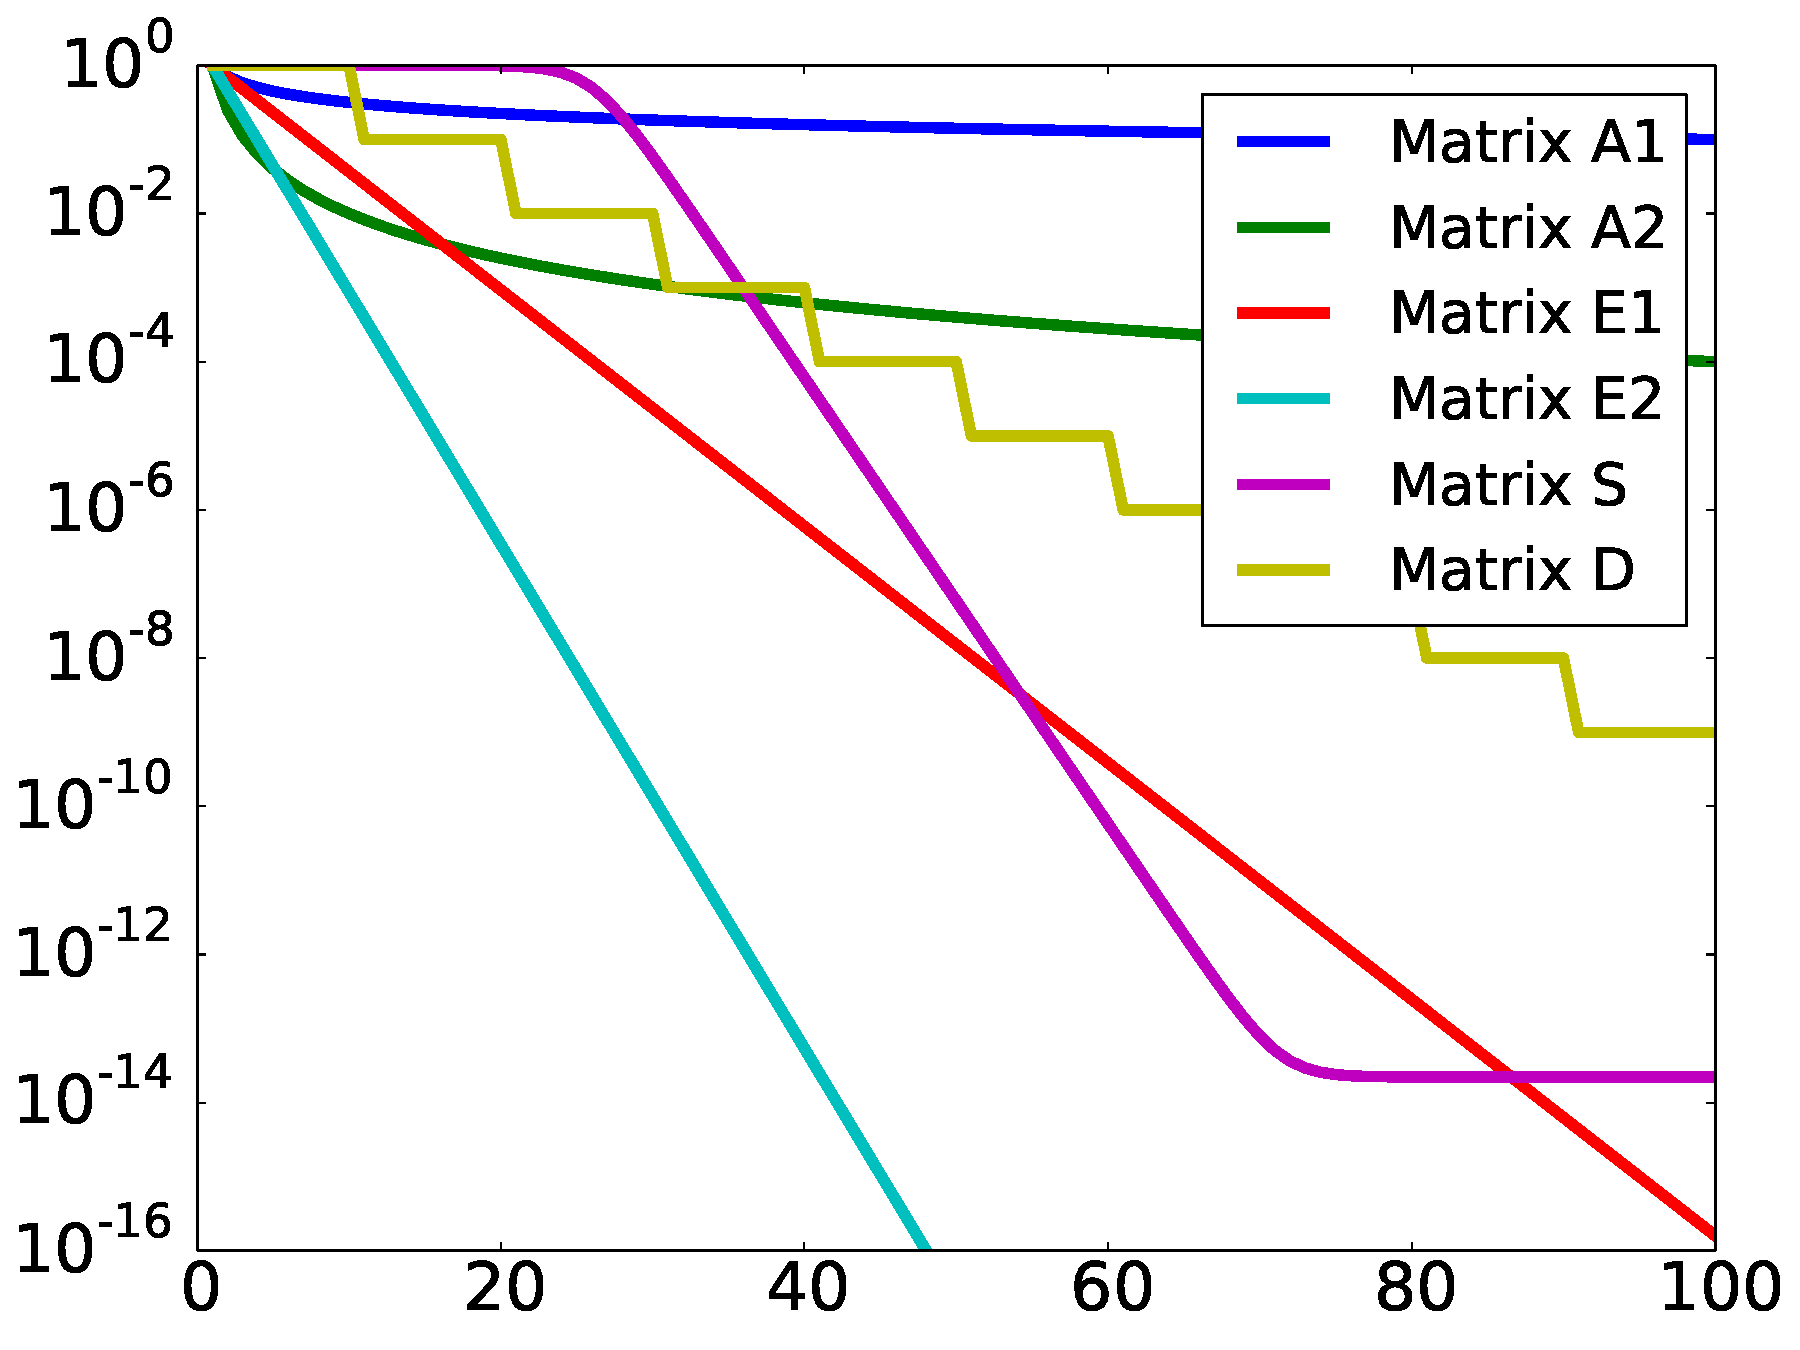
\includegraphics[width=8cm]{plots/sing_value_plot_dis.pdf}
\caption[Matrix Singular Values]{
A plot of the singular values for the matrices we
are investigating.}
\label{fig:sing_decay}
\end{figure}


\subsection{Norm Approximation}
% Give examples to show how HMT over estimates norm

We begin by showing how poorly the HMT error bound from
Lem.~\ref{thm:rand_hmt_bound} is by using it to estimate
$\norm{A}_{2}$; the results are shown
in Table~\ref{tab:hmt_norm_ubound_mat}, and we remember $\norm{A}_{2}\approx1$.
We let $\alpha\in\braces{2,5,10}$ and choose the number of samples
$p$ so that $\alpha^{p}\le 10^{-\ell}$ for various $\ell$.
To allow for comparisons, we let
$\alpha^{p}\in\braces{10^{-9},10^{-12},10^{-15}}$.
It is clear that in \emph{every} case the norm is overestimated, always
$3\times$ and frequently $10\times$ larger; furthermore, smaller $\alpha$
always leads to a more accurate estimate.
As we can see, we greatly overestimate the norm.
We are able to accurately measure the F-norm as seen
in Fig.~\ref{fig:geb_norm_bound_mat} using our stochastic estimate;
note the logarithmic scale on the number of columns ($d$).
We also include estimates of the squared F-norm in
Fig.~\ref{fig:geb_norm_squared_bound_mat} including mean and standard
deviations as well as the theoretical standard deviations;
the predicted results accurately match expected results.
We averaged 10,000 trials to obtain the statistics for these results.
In order to obtain the theoretical standard deviations in
Fig.~\ref{fig:geb_norm_squared_bound_mat}, we took the square root
of the variance from Eq.~\eqref{eq:rand_Xd_variance_bounds}.

%%%%%%%%%%%%%%%%%%%%%%%%%%%%%%%%%%%%%%%%%%%%%%%%%%%%%%%%%%%%%%%%%%%%%%%%
%%% Table of Upper Bounds for 2-Norm estimates

\begin{table}
\begin{center}
\begin{tabular}{cc|c|c|c|c|c|c|c|c|c|}
\cline{3-11}
& & \multicolumn{3}{|c|}{\textbf{1E-9}} &
\multicolumn{3}{|c|}{\textbf{1E-12}} & \multicolumn{3}{|c|}{\textbf{1E-15}} \\
\cline{3-11}
& & $p$ & M & S & $p$ & M & S & $p$ & M & S \\
\hline
\multicolumn{1}{|c|}{\multirow{3}{*}{Matrix A1}} & \textbf{2} &
    30 & 5.11 & 0.53 & 40 & 5.23 & 0.52 & 50 & 5.32 & 0.52 \\
\cline{2-11}
\multicolumn{1}{|c|}{} &\textbf{5} &
    13 & 11.8 & 1.4 & 18 & 12.2 & 1.4 & 22 & 12.4 & 1.3 \\
\cline{2-11}
\multicolumn{1}{|c|}{} &\textbf{10} &
    9 & 22.9 & 2.8  & 12 & 23.5 & 2.8  & 15 & 24.1 & 2.7 \\
\hline
\hline
\multicolumn{1}{|c|}{\multirow{3}{*}{Matrix A2}} & \textbf{2} &
    30 & 3.73 & 0.71 & 40 & 3.90 & 0.69 & 50 & 4.03 & 0.68 \\
\cline{2-11}
\multicolumn{1}{|c|}{} & \textbf{5} &
    13 & 8.02 & 1.93 & 18 & 8.52 & 1.86 & 22 & 8.85 & 1.82 \\
\cline{2-11}
\multicolumn{1}{|c|}{} & \textbf{10} &
    9 & 14.8 & 4.0  & 12 & 15.8 & 3.9  & 15 & 16.5 & 3.8 \\
\hline
\hline
\multicolumn{1}{|c|}{\multirow{3}{*}{Matrix E1}} & \textbf{2} &
    30 & 4.11 & 0.64 & 40 & 4.26 & 0.63 & 50 & 4.38 & 0.62 \\
\cline{2-11}
\multicolumn{1}{|c|}{} & \textbf{5} &
    13 & 9.14  & 1.72  & 18 & 9.58  & 1.68  & 22 & 9.86  & 1.66 \\
\cline{2-11}
\multicolumn{1}{|c|}{} & \textbf{10} &
    9 & 17.2 & 3.6   & 12 & 18.0  & 3.5  & 15 & 18.7 & 3.4 \\
\hline
\hline
\multicolumn{1}{|c|}{\multirow{3}{*}{Matrix E2}} & \textbf{2} &
    30 & 3.81 & 0.70 & 40 & 3.98 & 0.68 & 50 & 4.10 & 0.67 \\
\cline{2-11}
\multicolumn{1}{|c|}{} & \textbf{5} &
    13 & 8.27  & 1.90  & 18 & 8.78  & 1.83  & 22 & 9.07  & 1.79 \\
\cline{2-11}
\multicolumn{1}{|c|}{} & \textbf{10} &
    9 & 15.3 & 3.94   & 12 & 16.3  & 3.84  & 15 & 17.0 & 3.74 \\
\hline
\hline
\multicolumn{1}{|c|}{\multirow{3}{*}{Matrix S}} & \textbf{2} &
    30 & 10.1 & 0.6 & 40 & 10.2 & 0.6 & 50 & 10.3 & 0.6 \\
\cline{2-11}
\multicolumn{1}{|c|}{} & \textbf{5} &
    13 & 24.1  & 1.6  & 18 & 24.5  & 1.6  & 22 & 24.8  & 1.5 \\
\cline{2-11}
\multicolumn{1}{|c|}{} & \textbf{10} &
    9 & 47.0 & 3.5   & 12 & 47.9  & 3.3  & 15 & 48.5 & 3.2 \\
\hline
\hline
\multicolumn{1}{|c|}{\multirow{3}{*}{Matrix D}} & \textbf{2} &
    30 & 7.36 & 0.64 & 40 & 7.51 & 0.61 & 50 & 7.61 & 0.60 \\
\cline{2-11}
\multicolumn{1}{|c|}{} & \textbf{5} &
    13 & 17.2  & 1.8  & 18 & 17.7  & 1.7  & 22 & 18.0  & 1.6 \\
\cline{2-11}
\multicolumn{1}{|c|}{} & \textbf{10} &
    9 & 33.3 & 3.7   & 12 & 34.2  & 3.6  & 15 & 34.8 & 3.5 \\
\hline
\end{tabular}
\end{center}
\caption[HMT 2-Norm Upper Bounds]{
Upper bound of $||A||_{2}$ based on
 Lemma~\ref{thm:rand_hmt_bound} (HMT) for different
failure probabilities (columns) and $\alpha$ (rows).
$p$ is the smallest integer for which $\alpha^{-p}\le 10^{-\ell}$.
We performed 10,000 trials and computed the mean (M) and standard deviation
(S). The correct values are $||A||_{2}\approx1$.
}
\label{tab:hmt_norm_ubound_mat}
\end{table}

% Print results for GEB estimates for F-norm

\begin{figure}[p]
    \centering

    \begin{subfigure}{0.45\textwidth}
    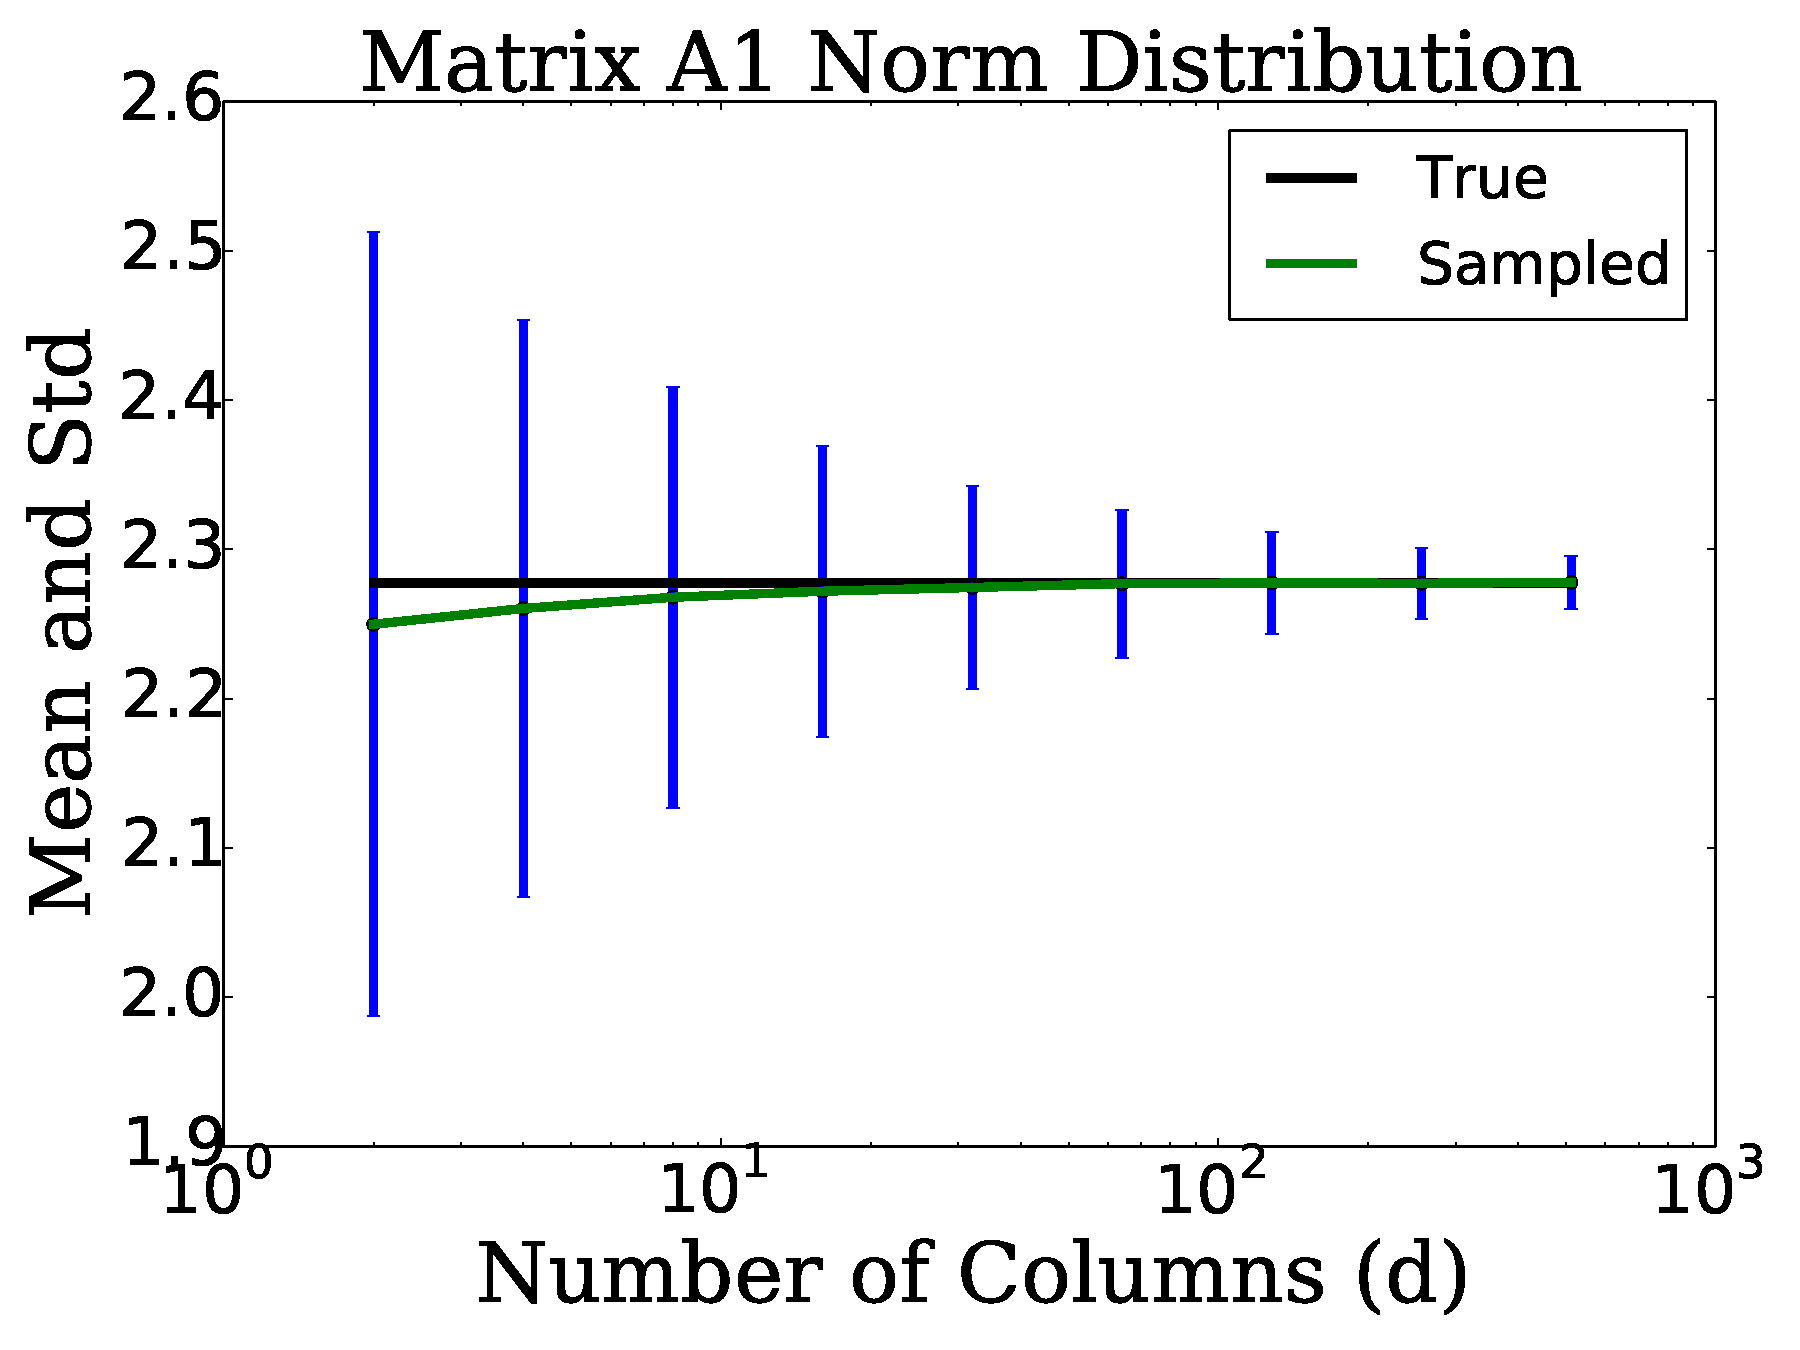
\includegraphics[width=\textwidth]{plots/mat_A1_error_test.pdf}
    \caption{Matrix A1}
    \end{subfigure}
    \begin{subfigure}{0.45\textwidth}
    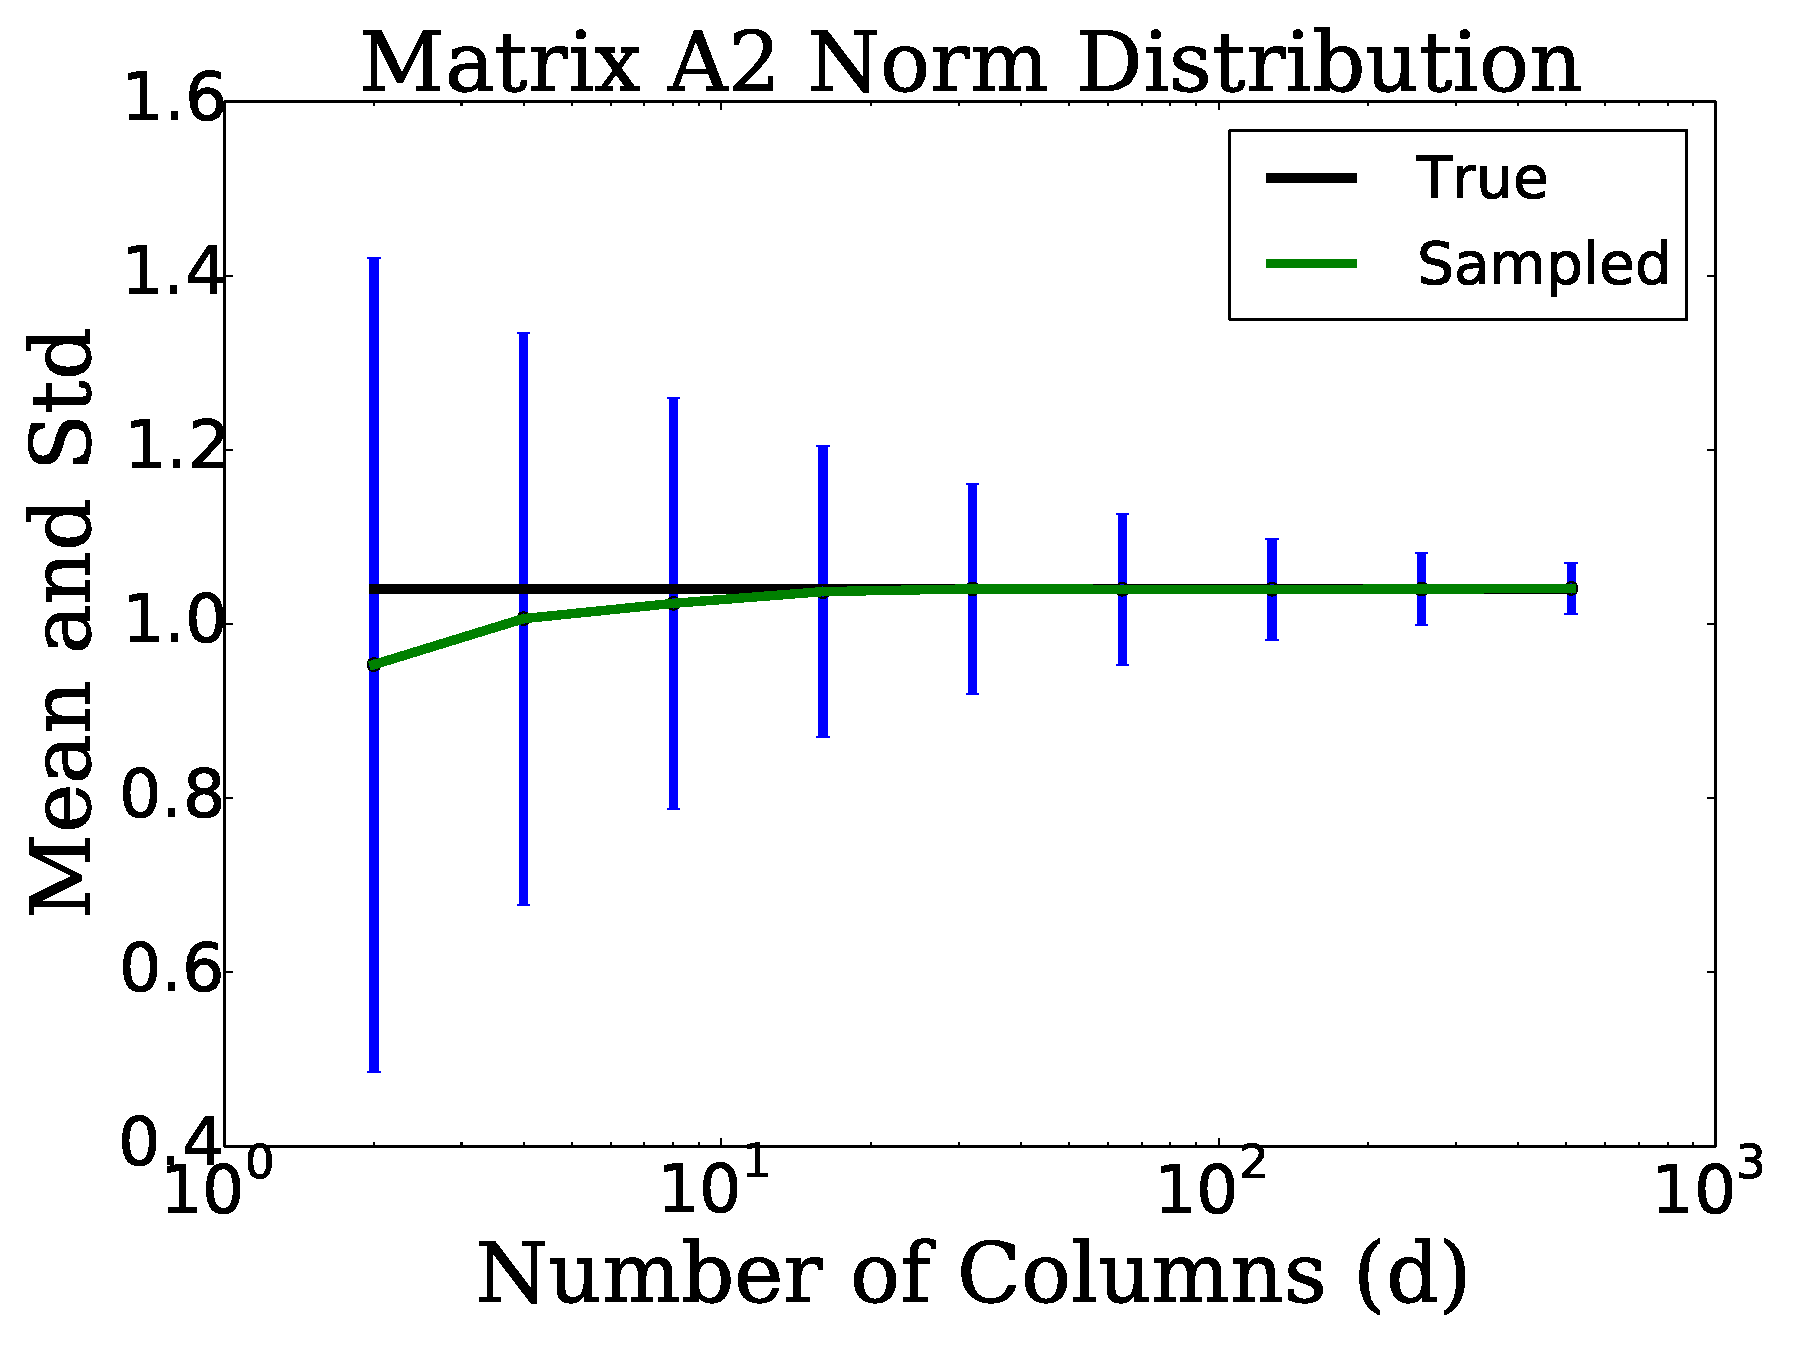
\includegraphics[width=\textwidth]{plots/mat_A2_error_test.pdf}
    \caption{Matrix A2}
    \end{subfigure}

    \begin{subfigure}{0.45\textwidth}
    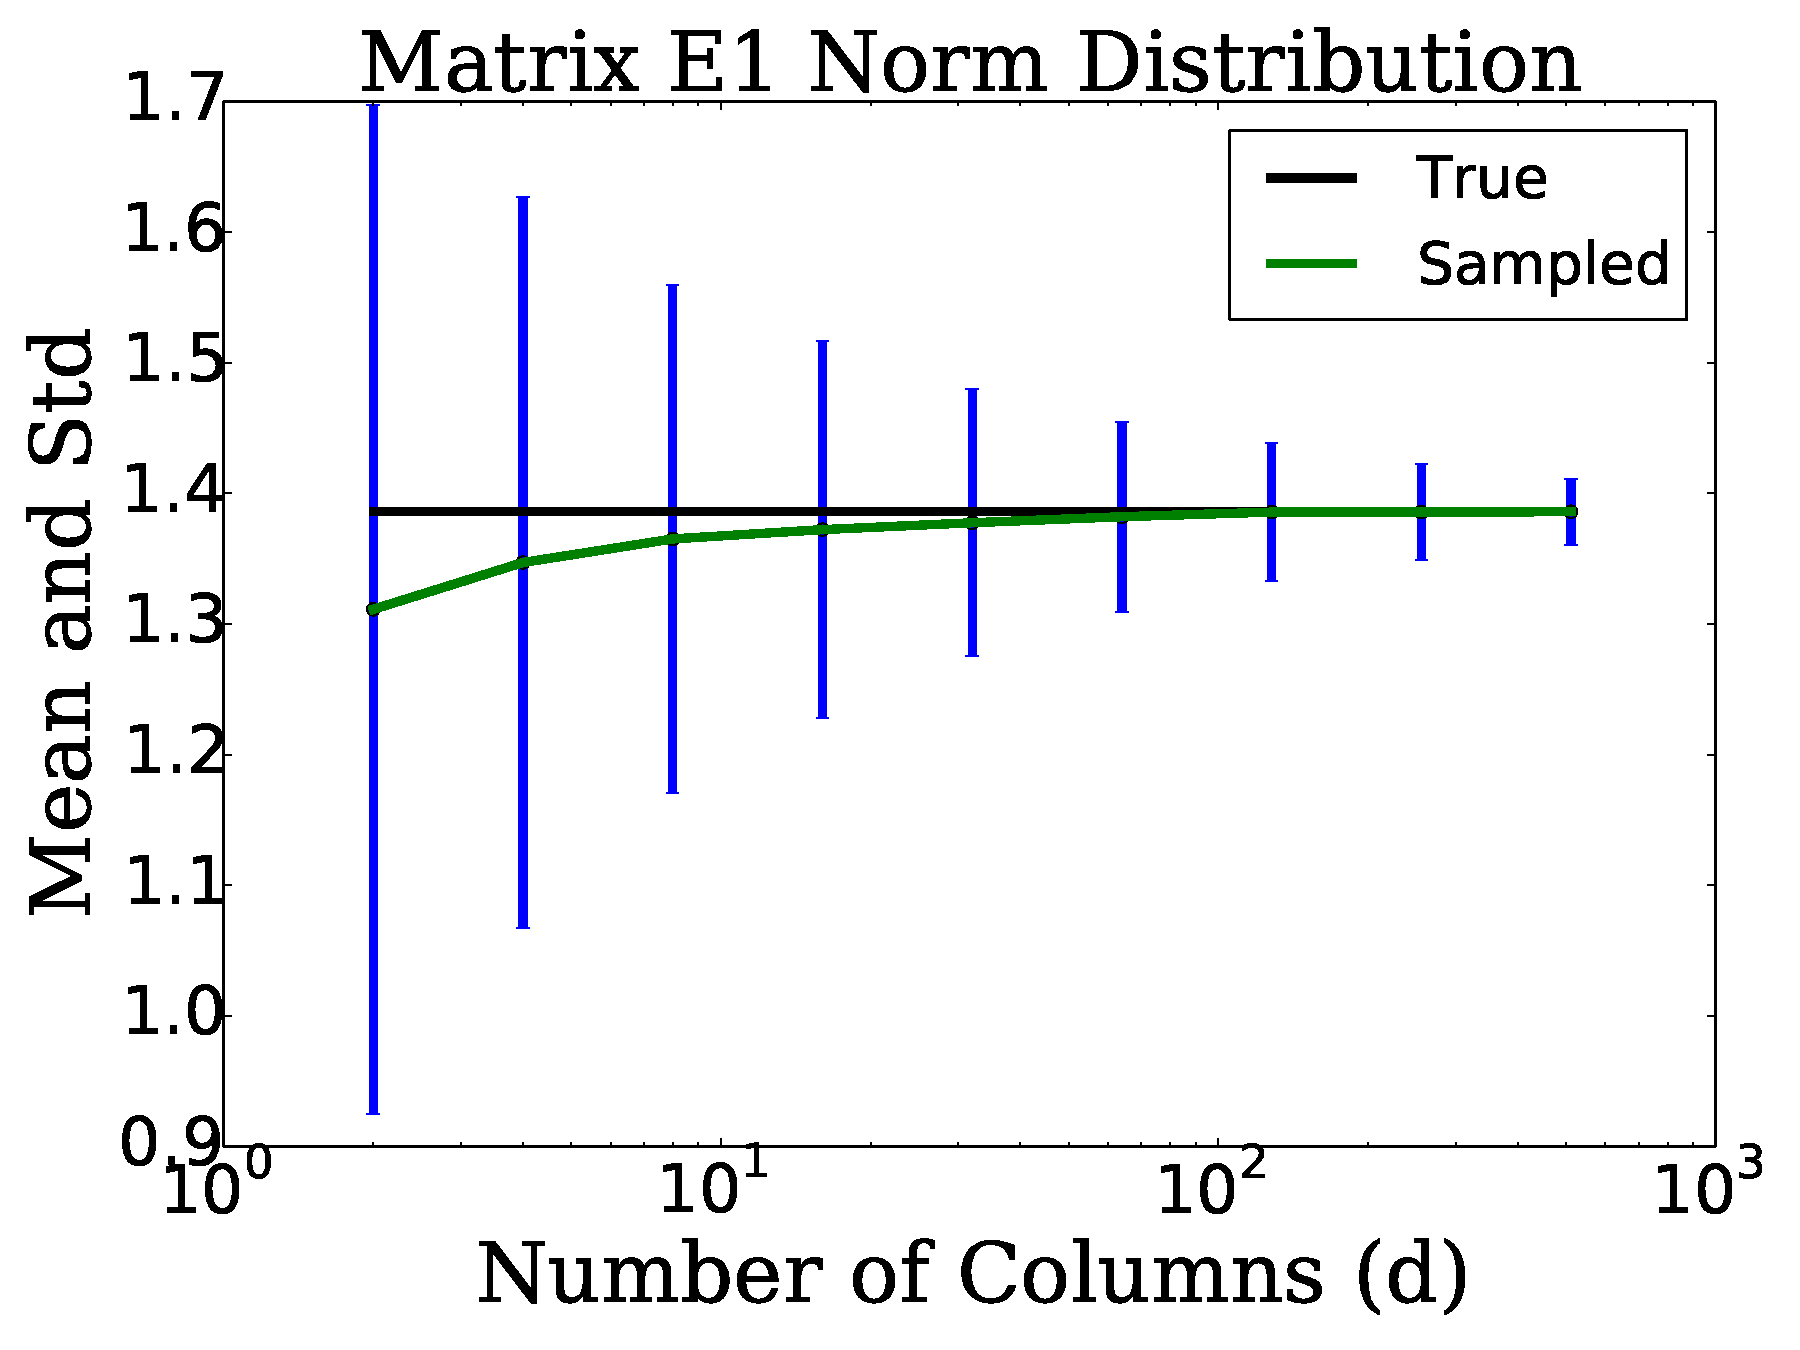
\includegraphics[width=\textwidth]{plots/mat_E1_error_test.pdf}
    \caption{Matrix E1}
    \end{subfigure}
    \begin{subfigure}{0.45\textwidth}
    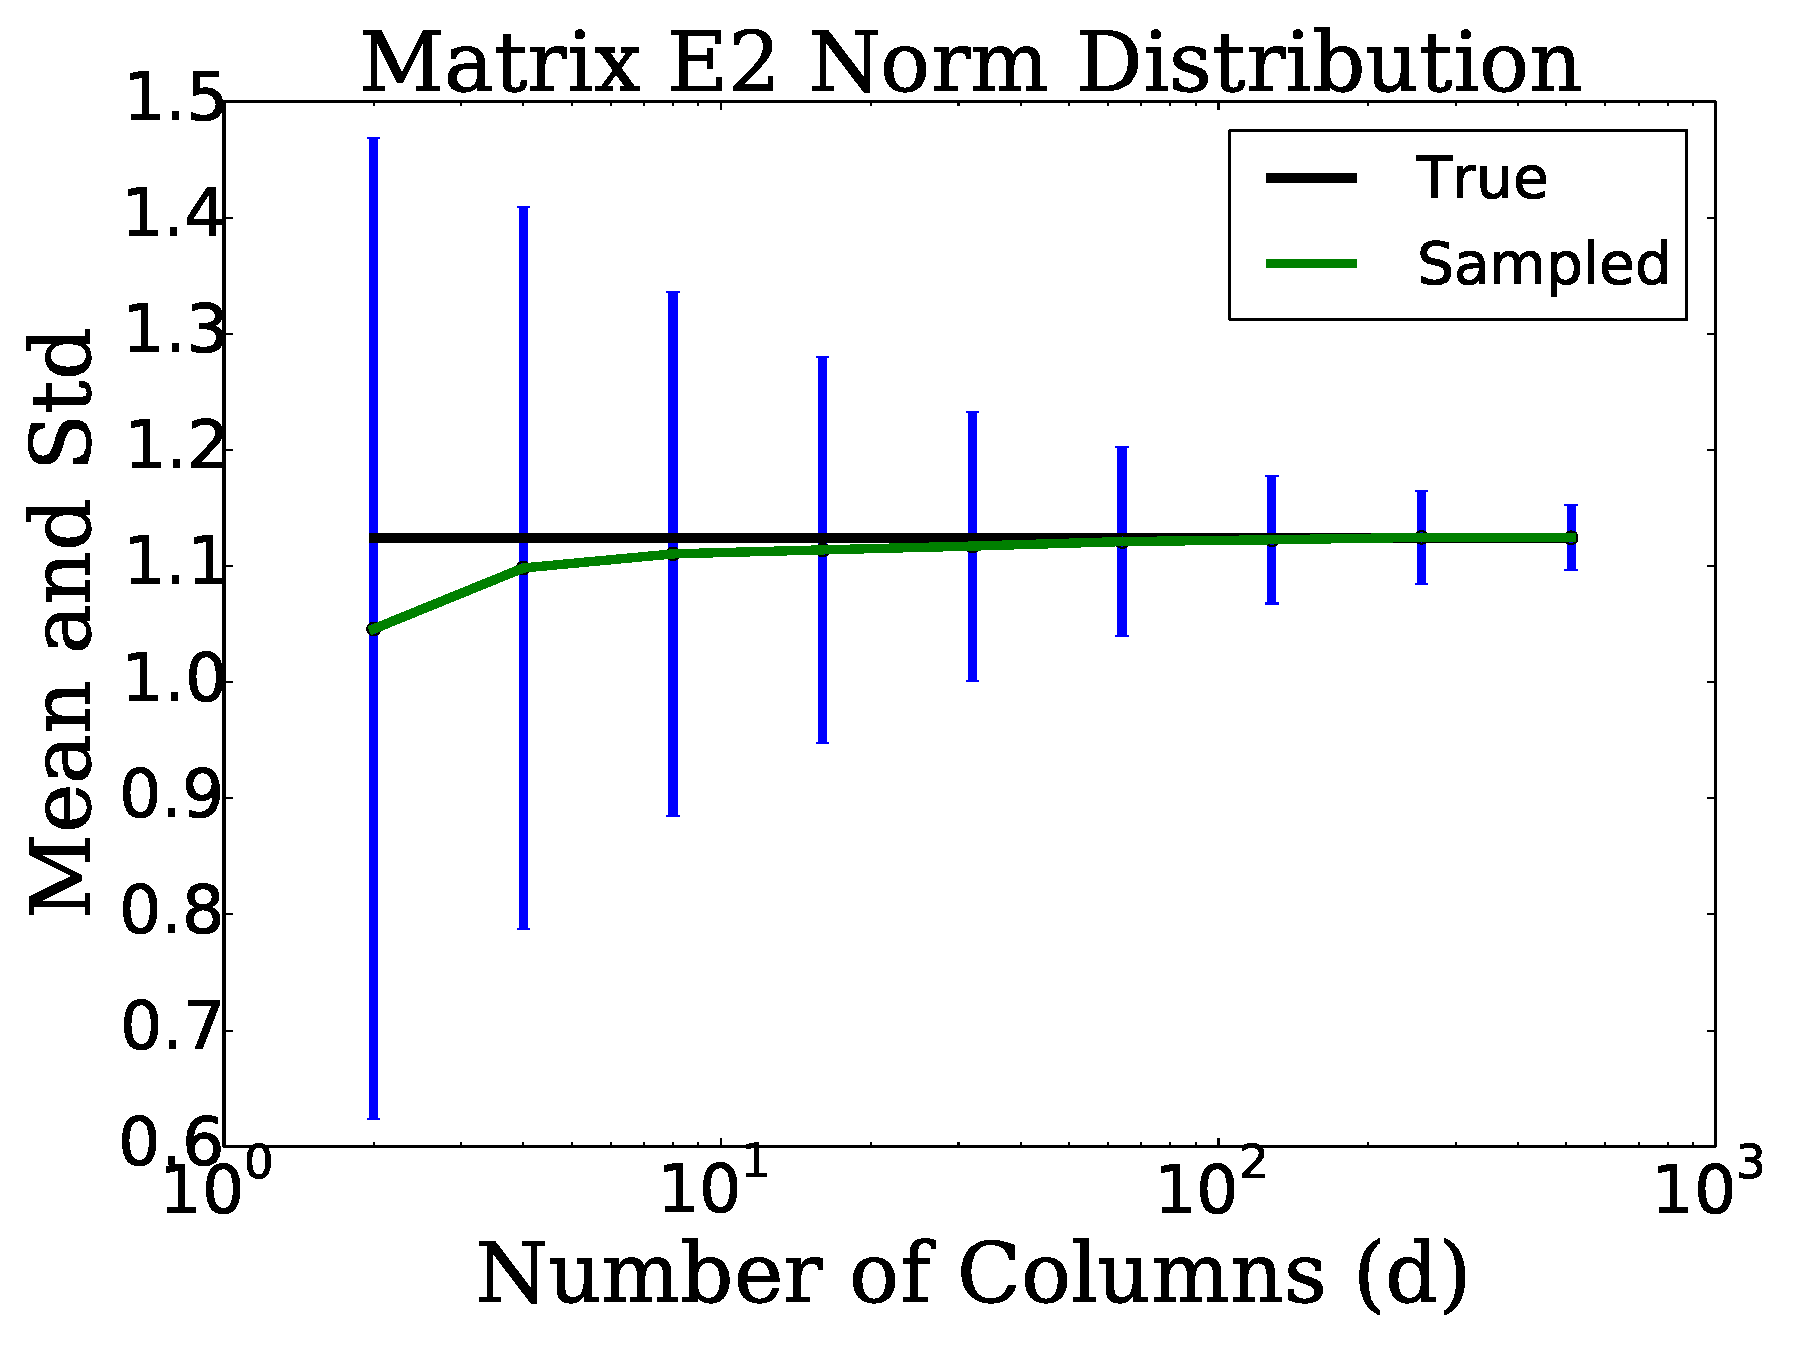
\includegraphics[width=\textwidth]{plots/mat_E2_error_test.pdf}
    \caption{Matrix E2}
    \end{subfigure}

    \begin{subfigure}{0.45\textwidth}
    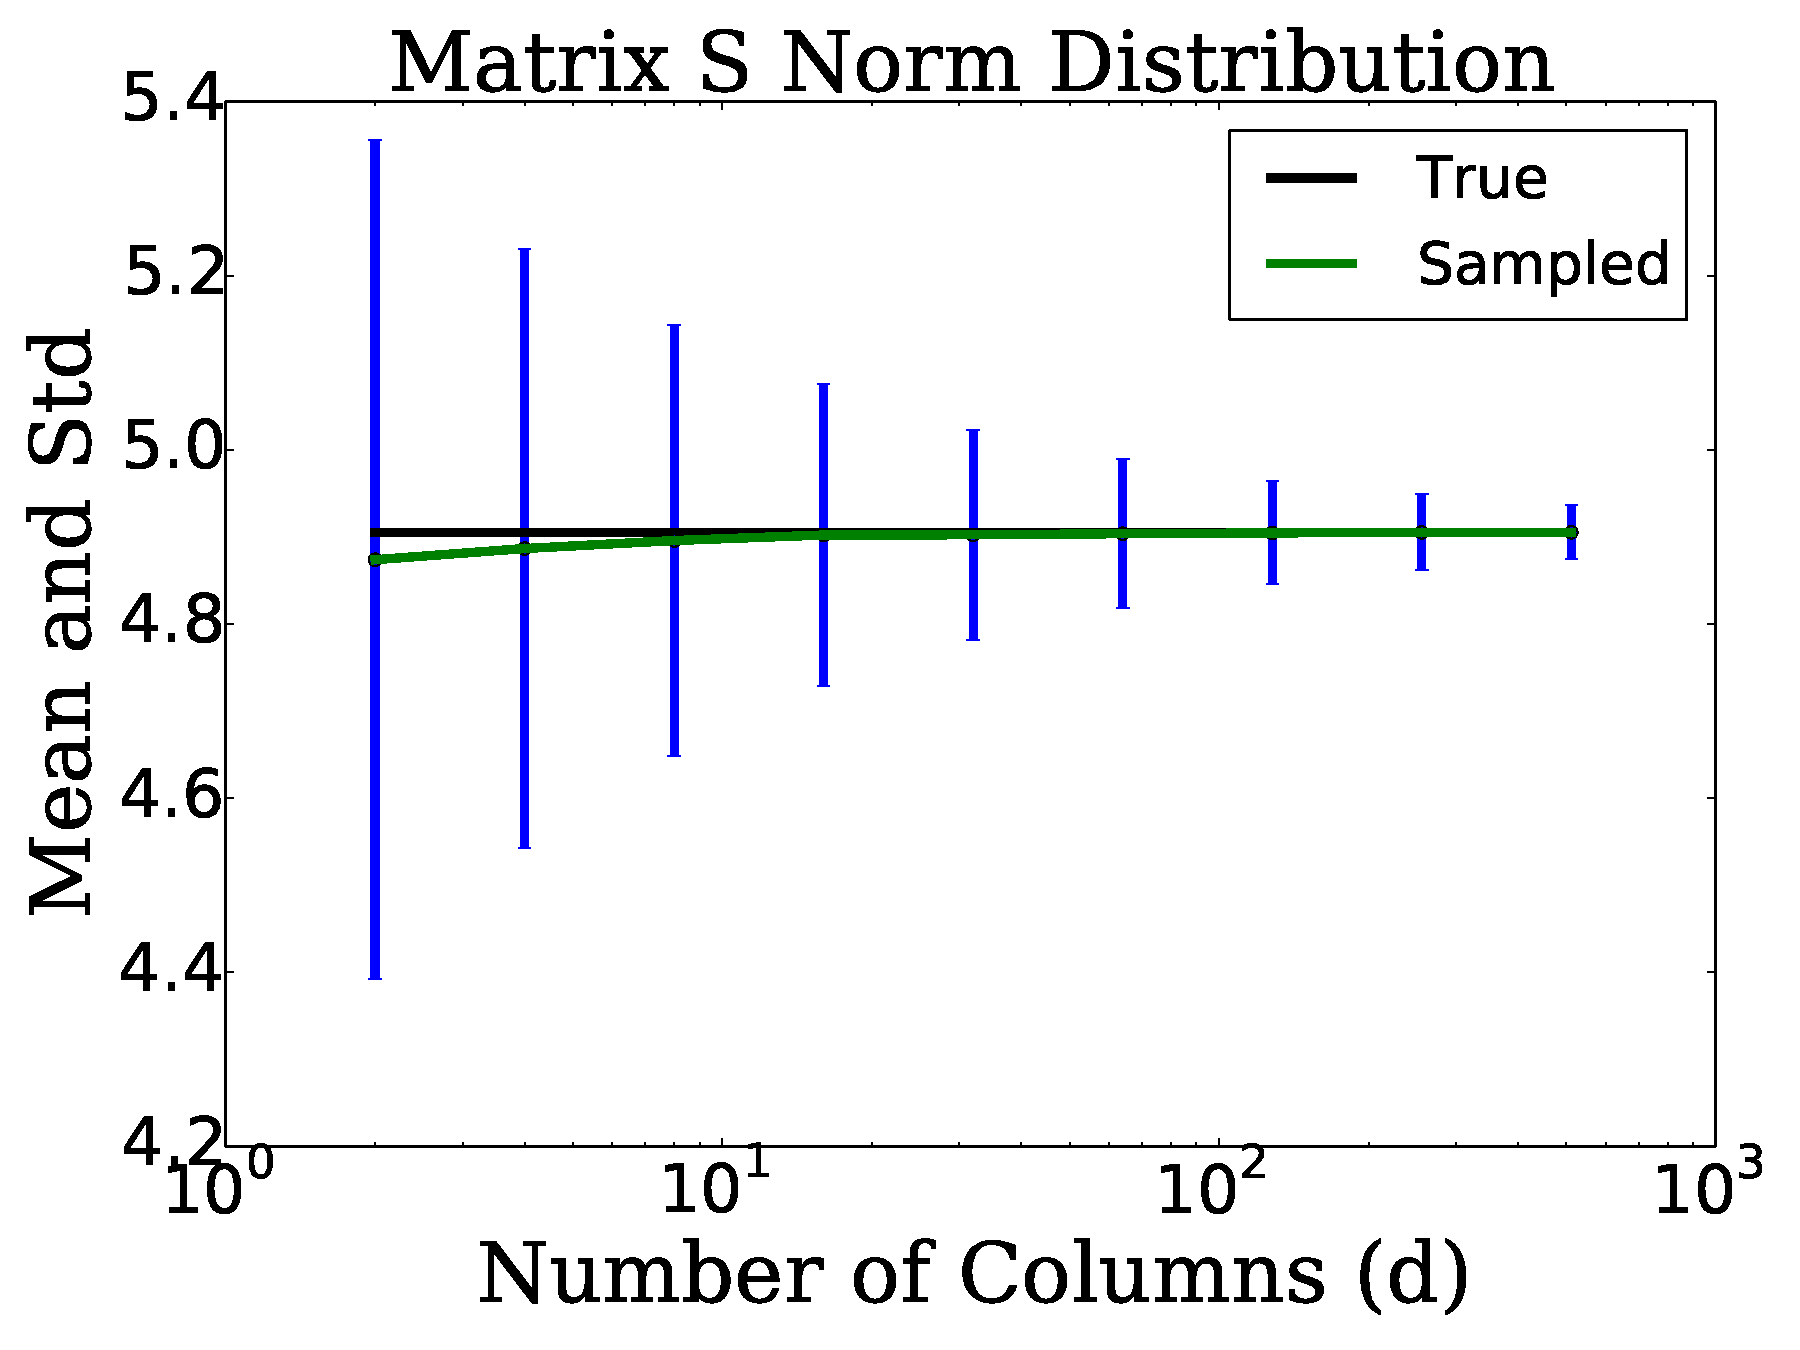
\includegraphics[width=\textwidth]{plots/mat_S_error_test.pdf}
    \caption{Matrix S}
    \end{subfigure}
    \begin{subfigure}{0.45\textwidth}
    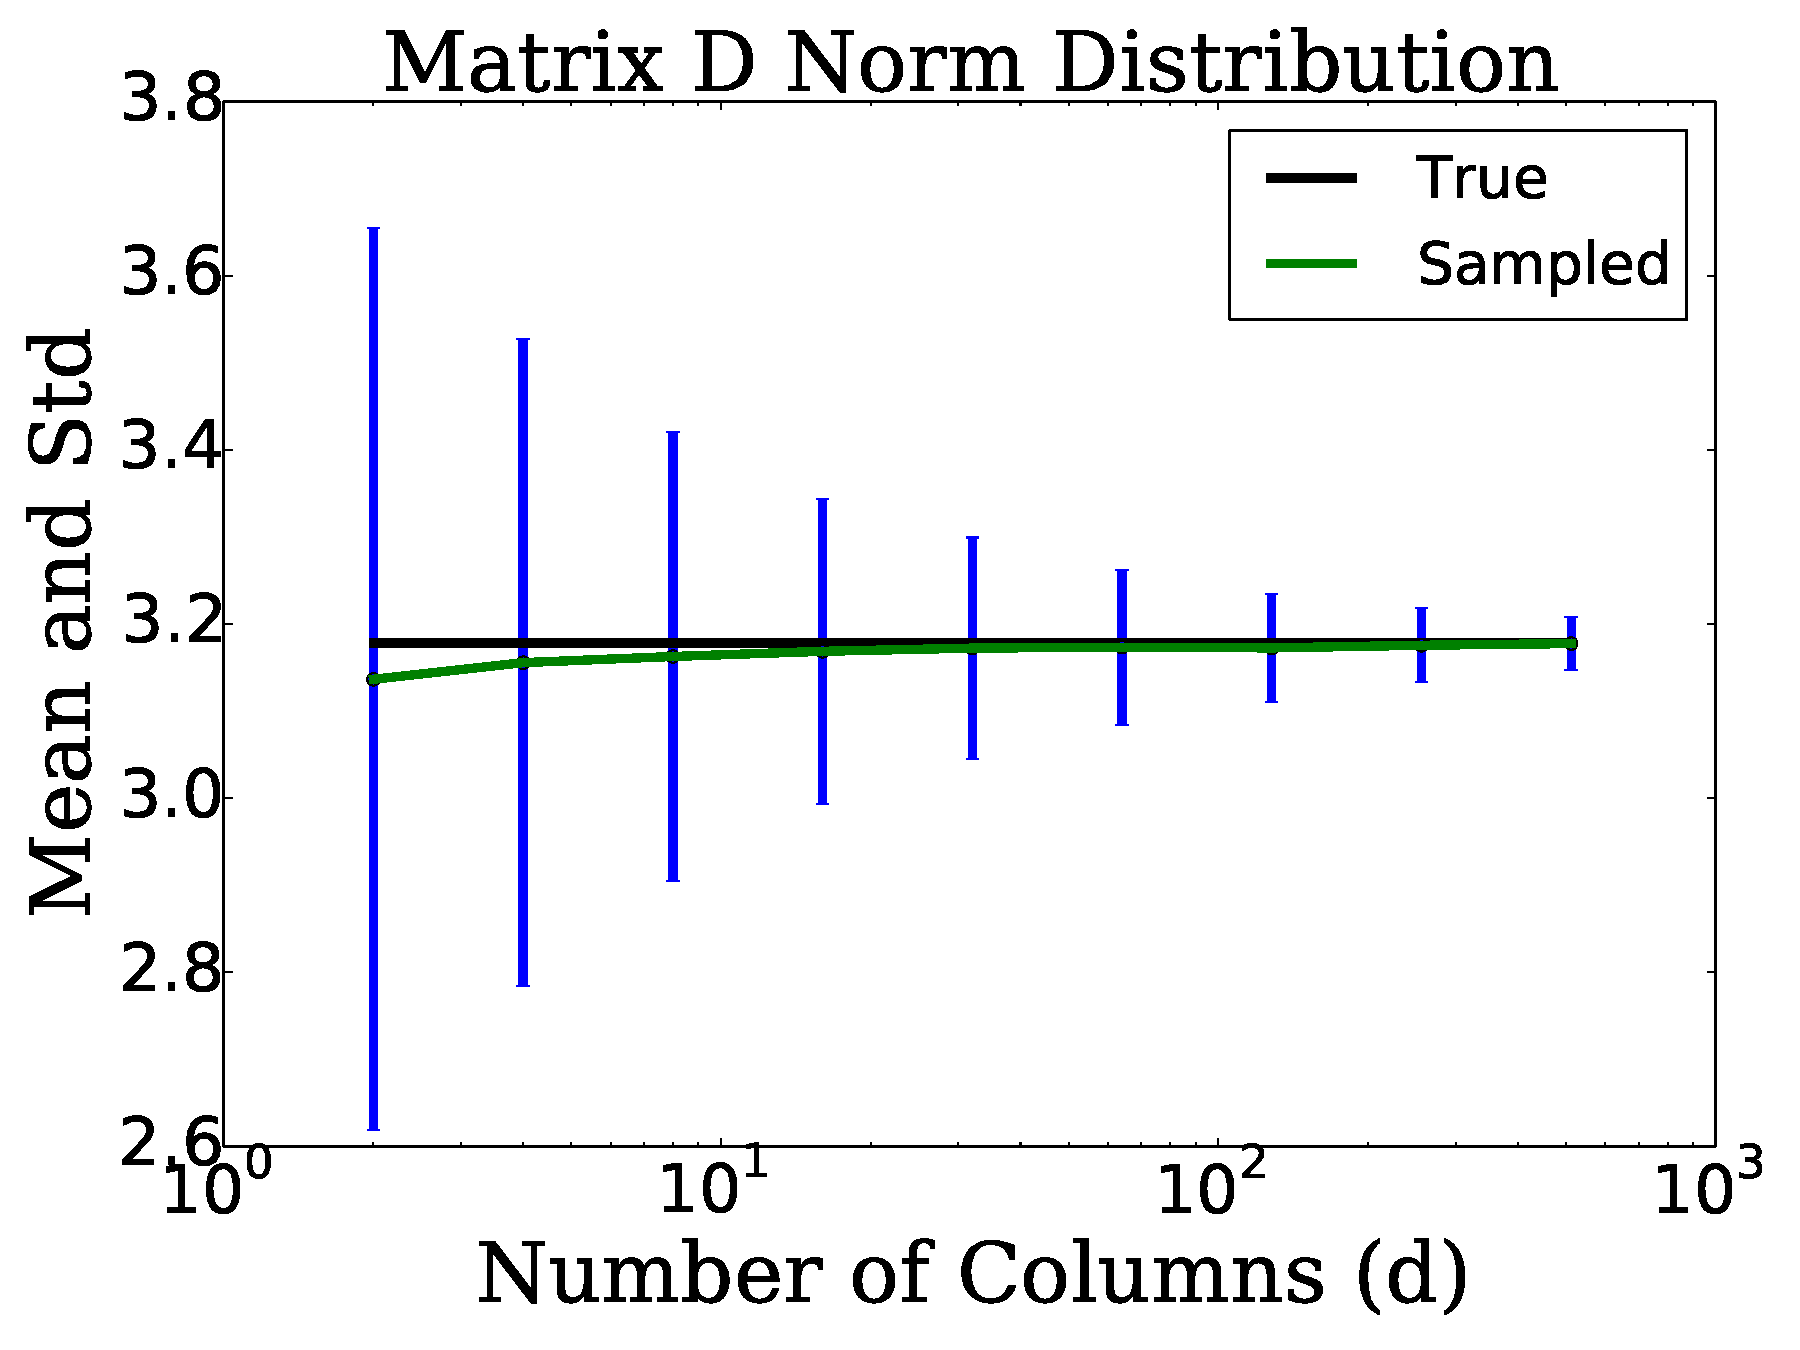
\includegraphics[width=\textwidth]{plots/mat_D_error_test.pdf}
    \caption{Matrix D}
    \end{subfigure}

\caption[GEB Stochastic F-norm Approximations]{
%Estimated $||A||_{F}$ for our matrices using the Gaussian Error Bound.
We performed 10,000 trials and computed the mean (Green) and
standard deviation (Blue) of $\norm{A\Omega}_{F}$ for columns
$d\in\{2,4,8,\cdots,512\}$.
The true F-norm value is Black.
}
\label{fig:geb_norm_bound_mat}
\end{figure}




% Print results for GEB estimates for F-norm^2

\begin{figure}[p]
    \centering

    \begin{subfigure}{0.45\textwidth}
    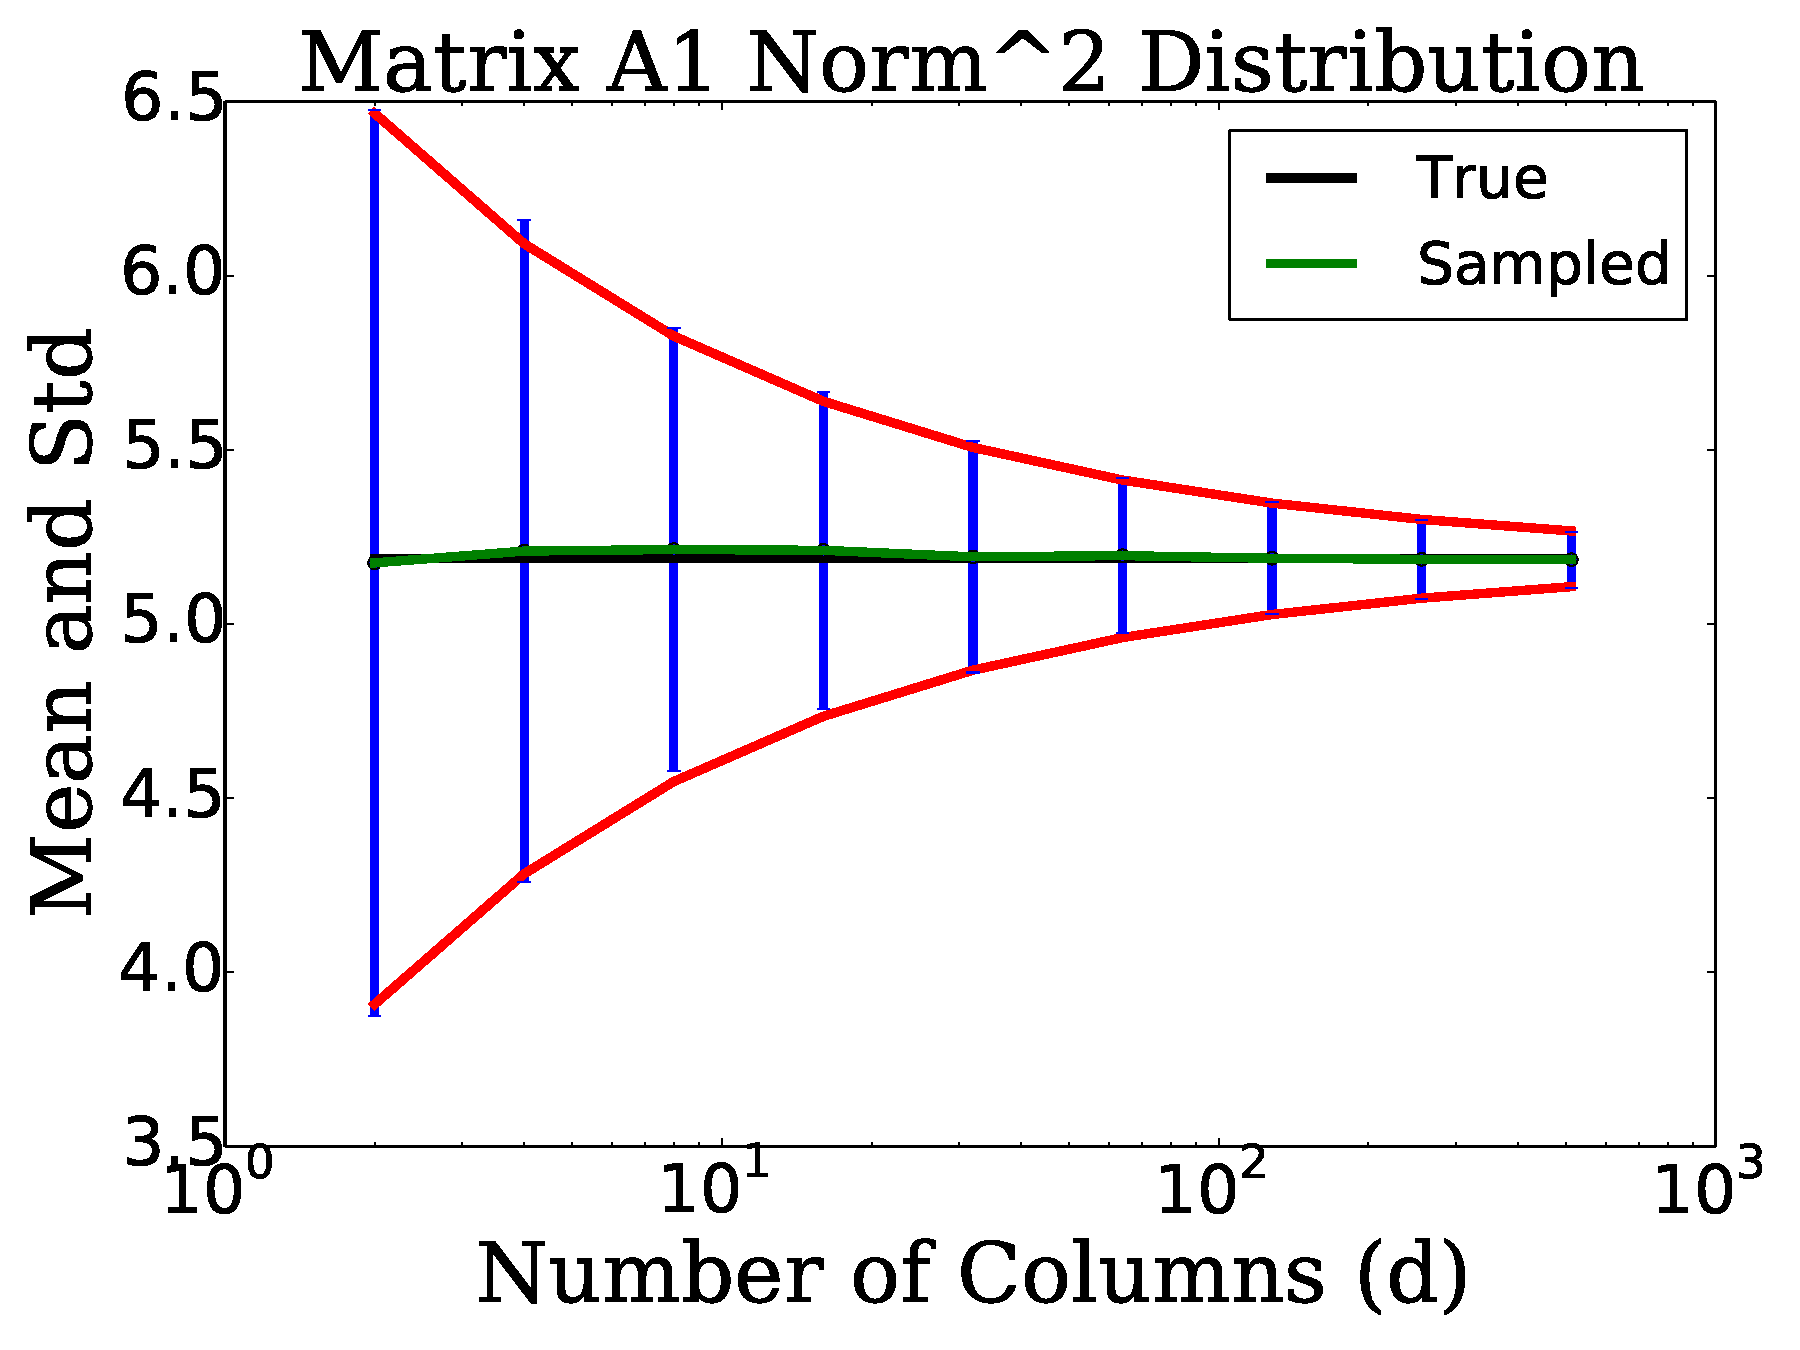
\includegraphics[width=\textwidth]{plots/mat_A1_error_test_2.pdf}
    \caption{Matrix A1}
    \end{subfigure}
    \begin{subfigure}{0.45\textwidth}
    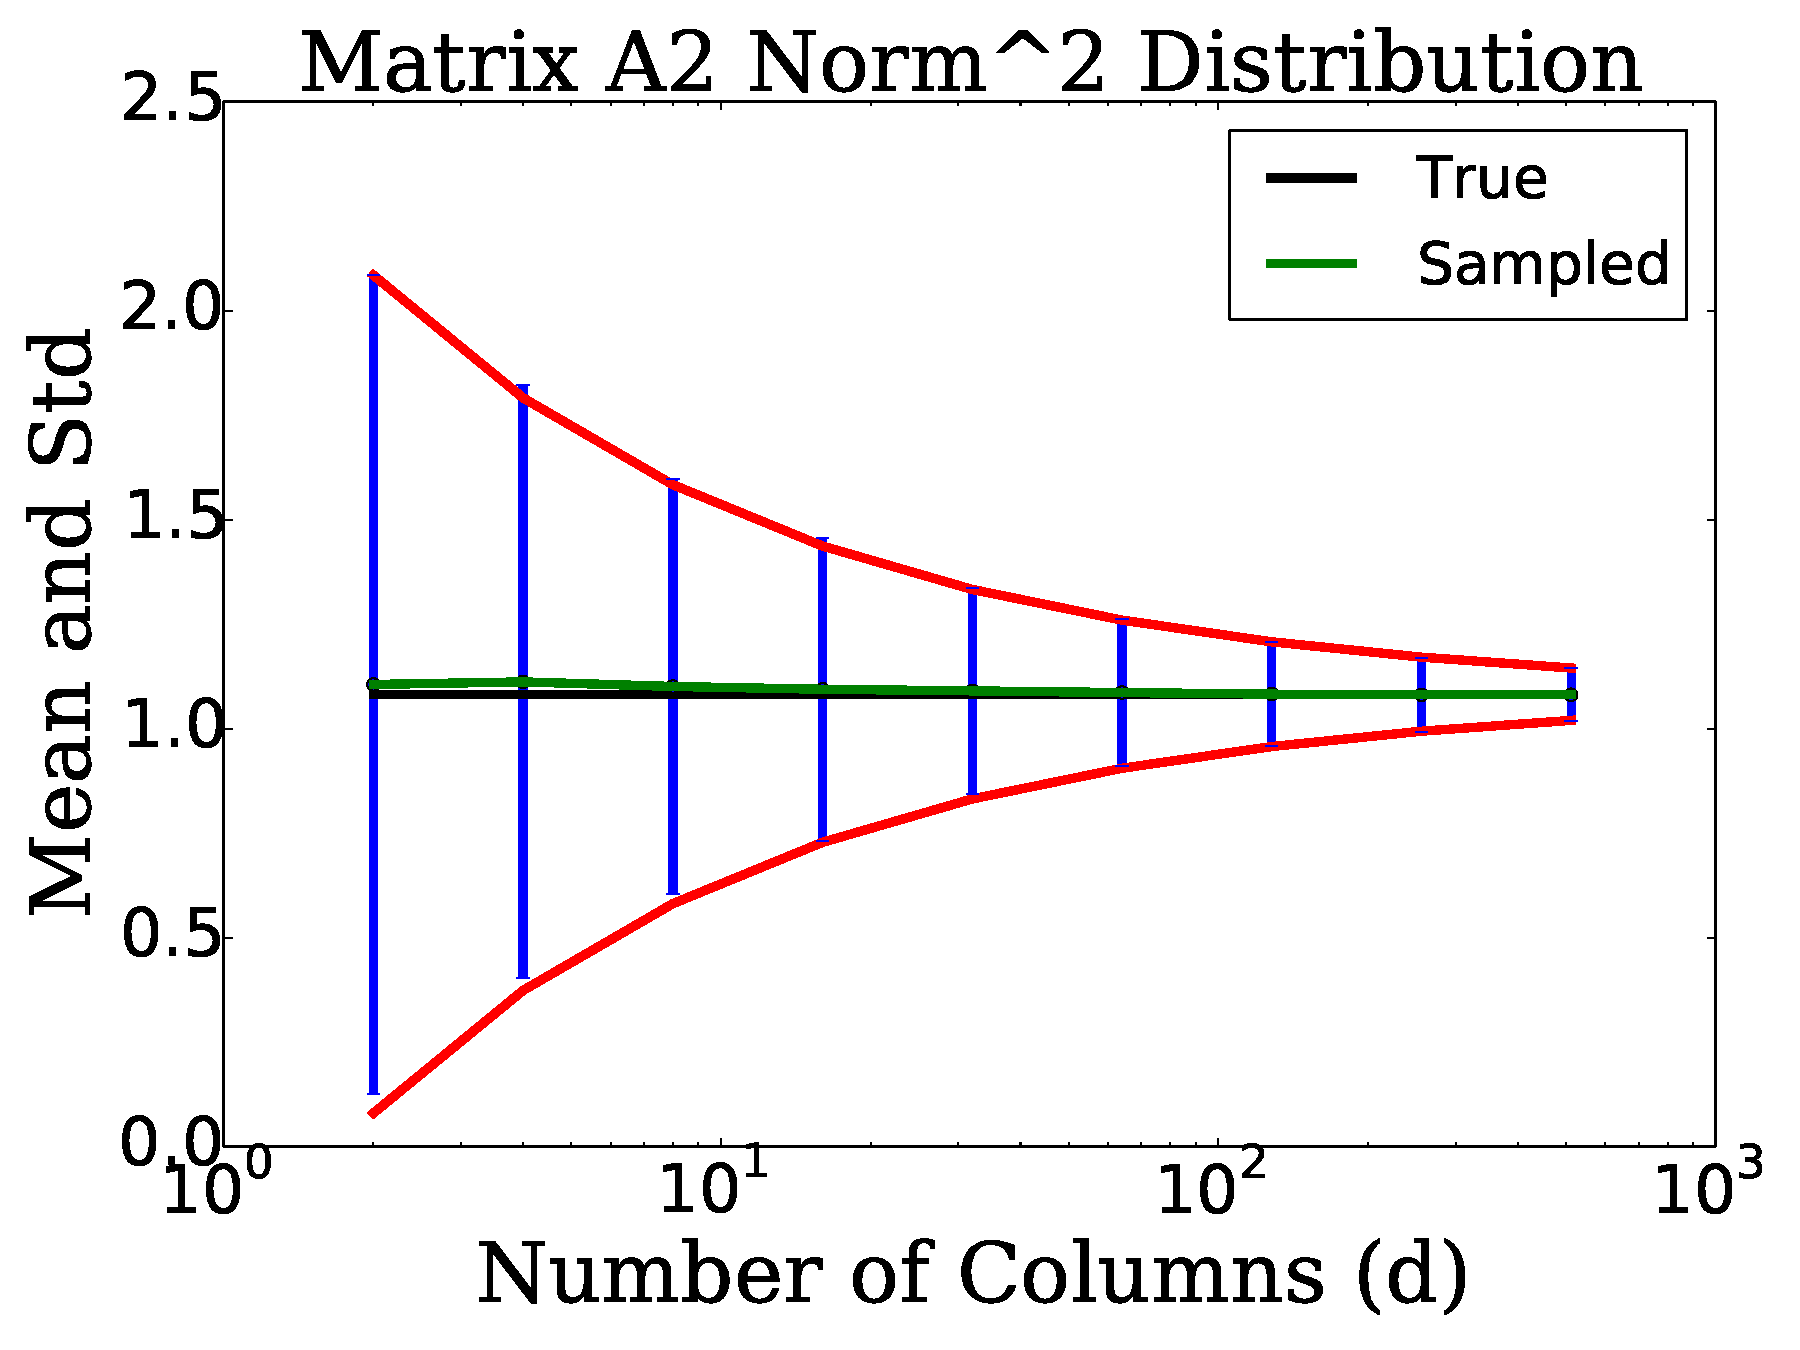
\includegraphics[width=\textwidth]{plots/mat_A2_error_test_2.pdf}
    \caption{Matrix A2}
    \end{subfigure}

    \begin{subfigure}{0.45\textwidth}
    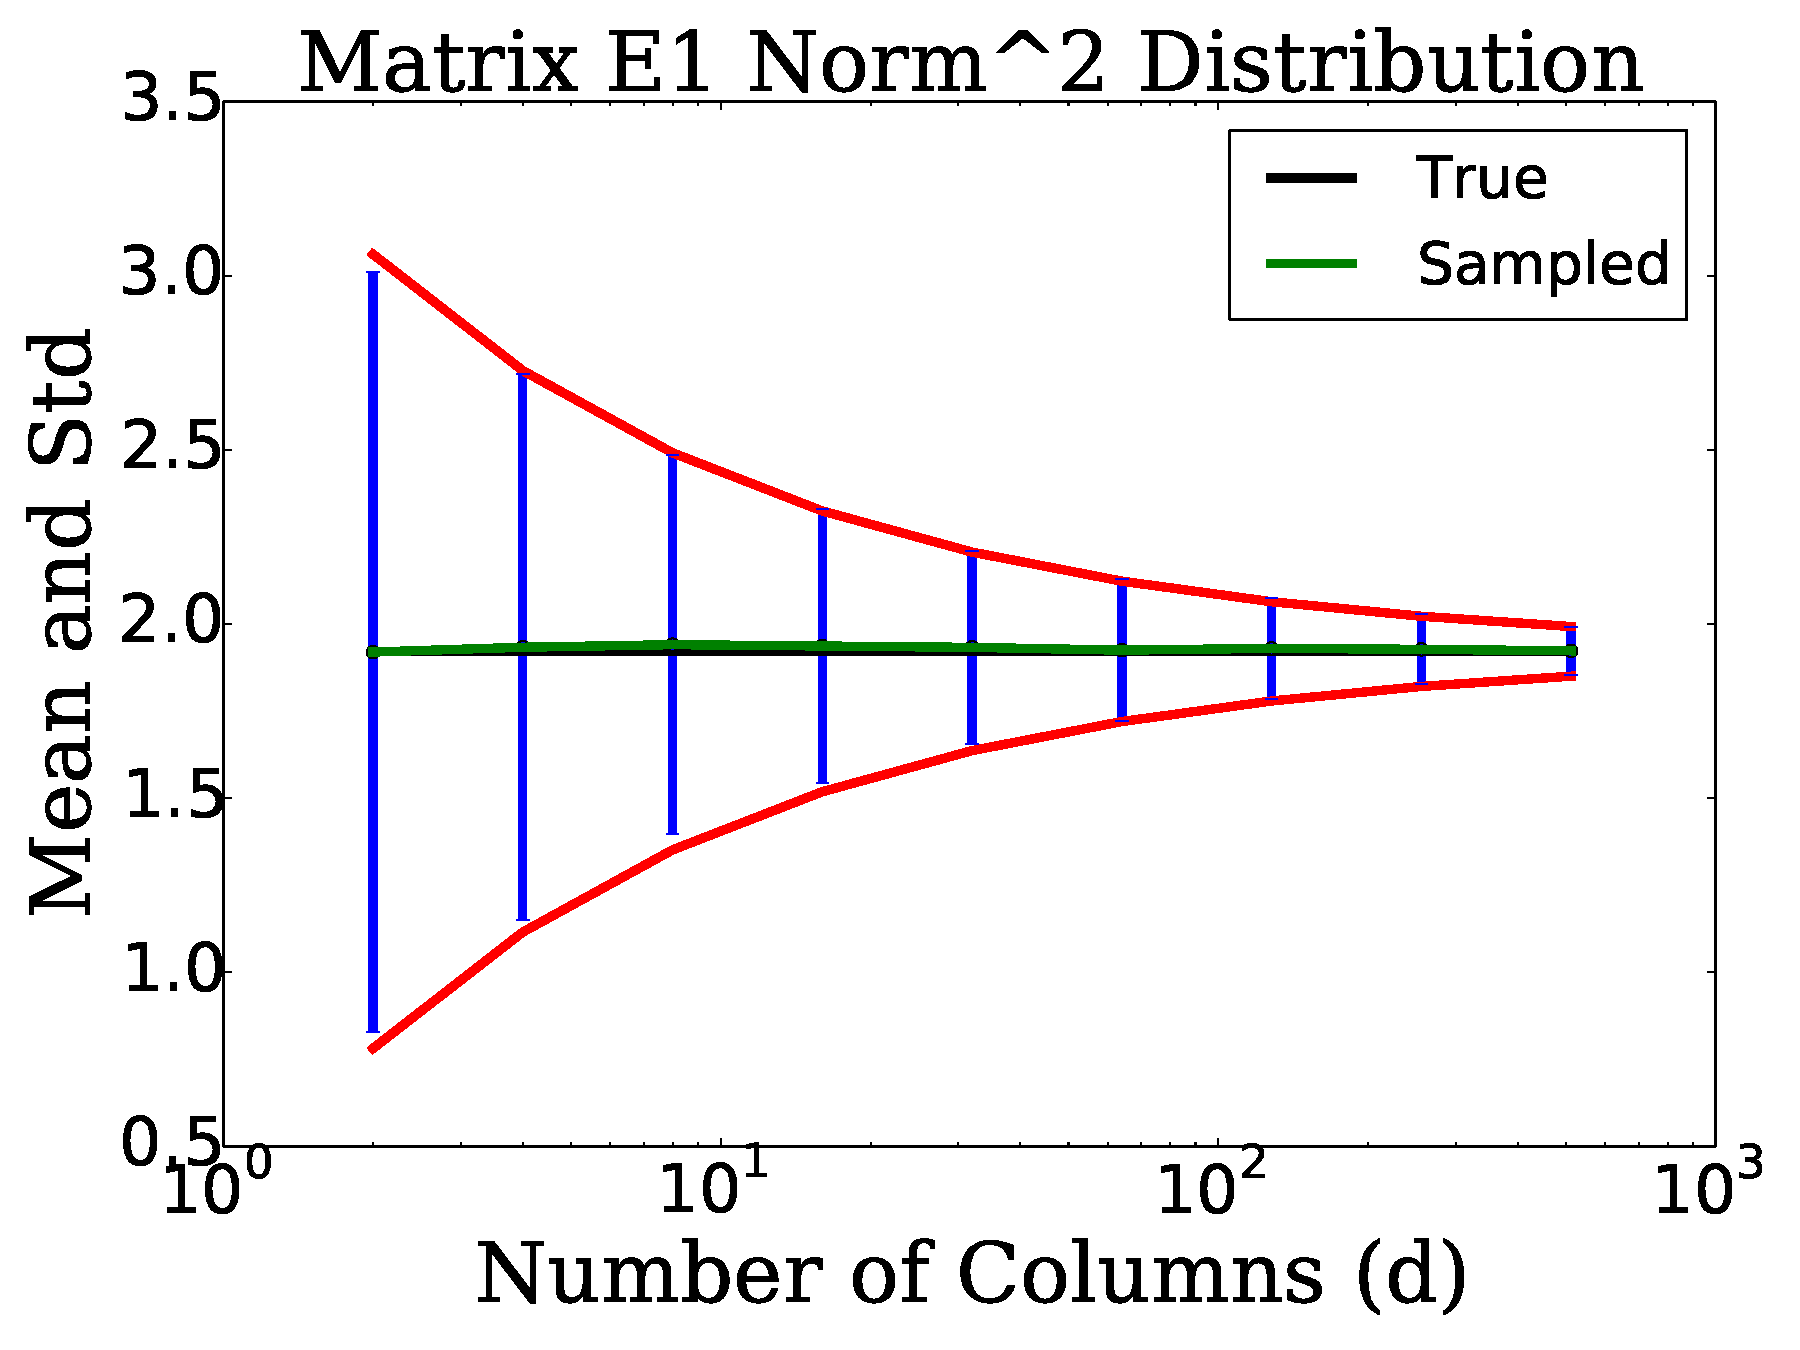
\includegraphics[width=\textwidth]{plots/mat_E1_error_test_2.pdf}
    \caption{Matrix E1}
    \end{subfigure}
    \begin{subfigure}{0.45\textwidth}
    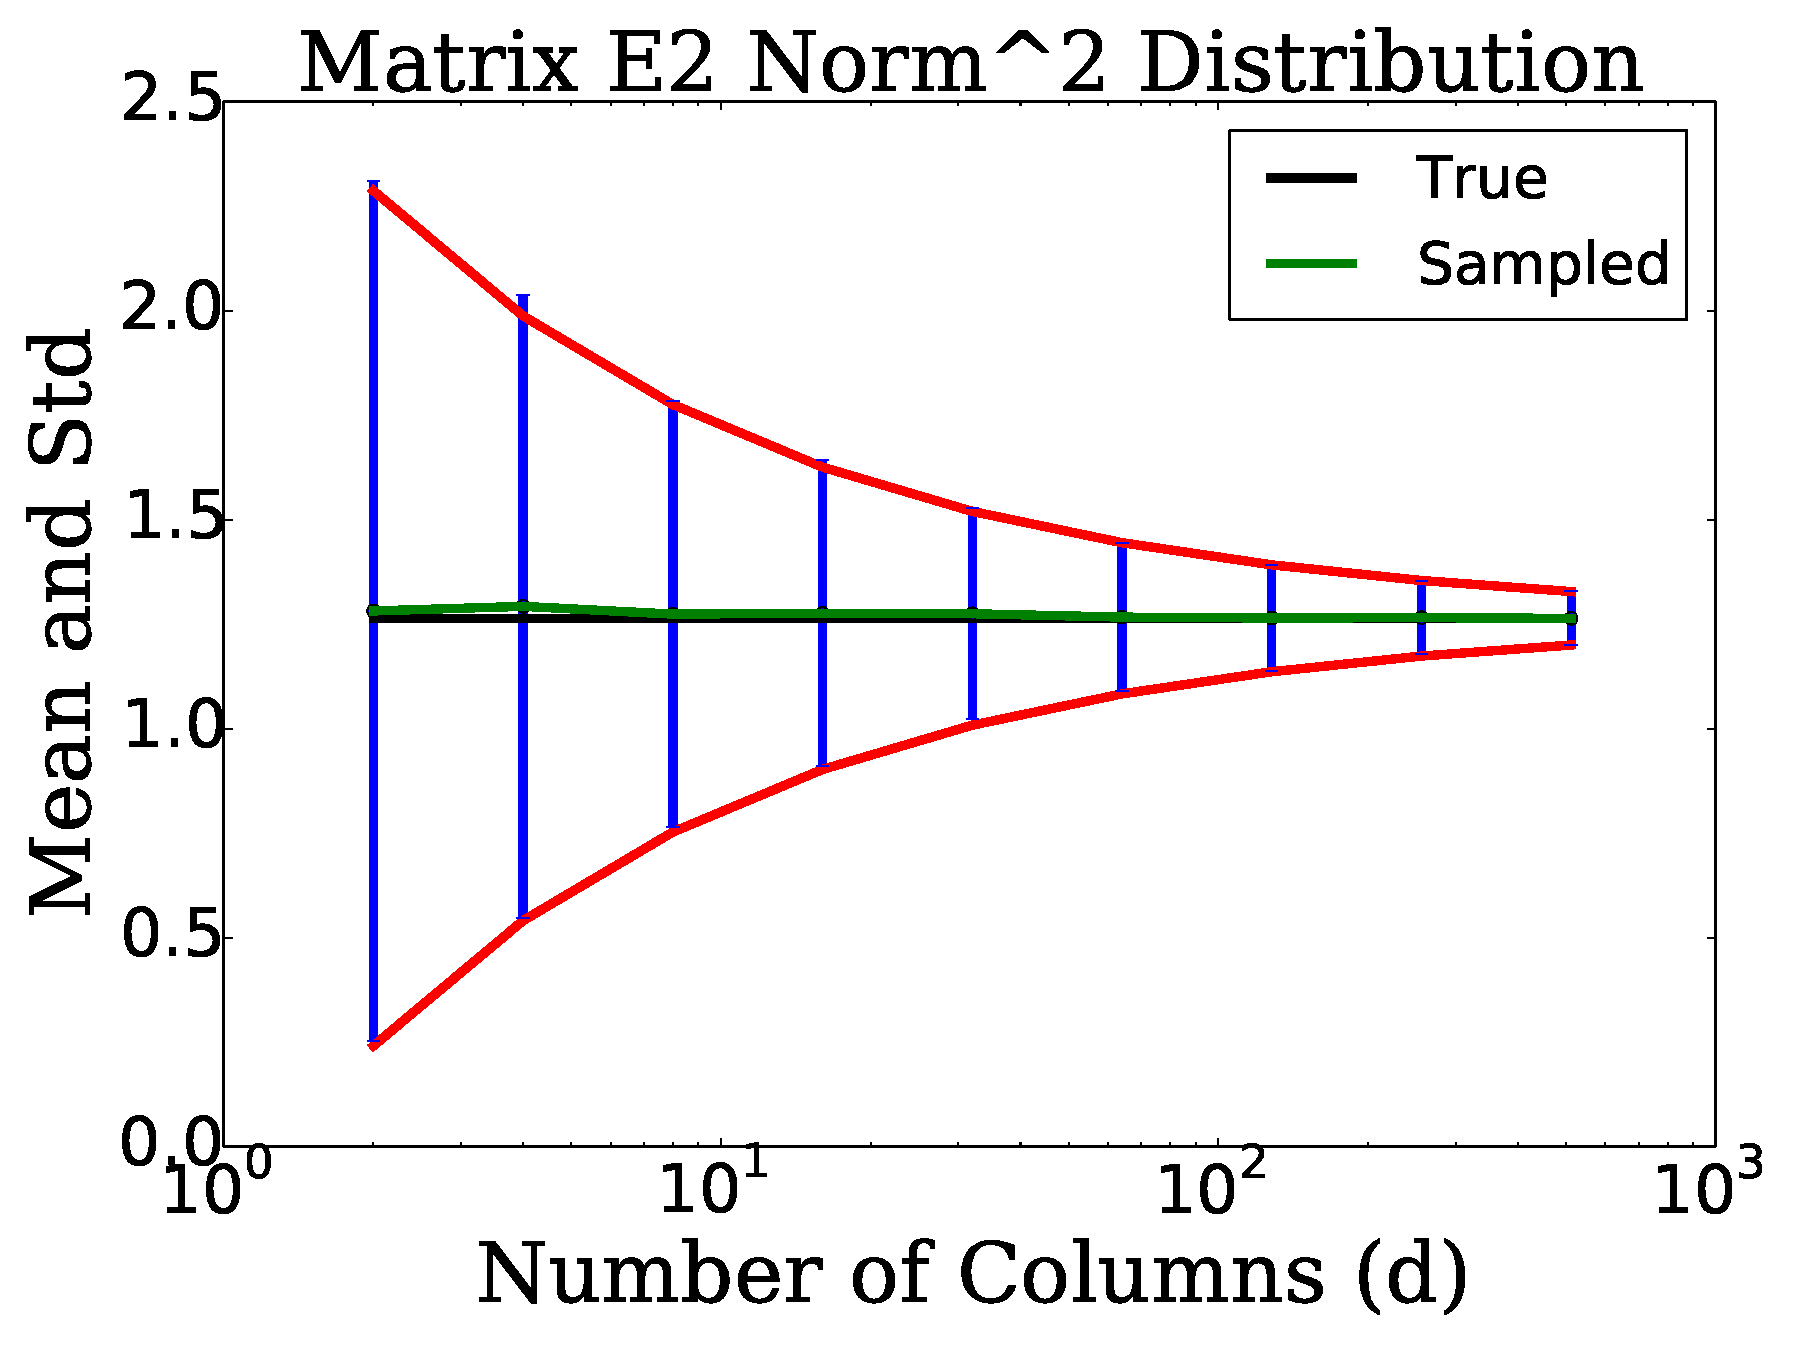
\includegraphics[width=\textwidth]{plots/mat_E2_error_test_2.pdf}
    \caption{Matrix E2}
    \end{subfigure}

    \begin{subfigure}{0.45\textwidth}
    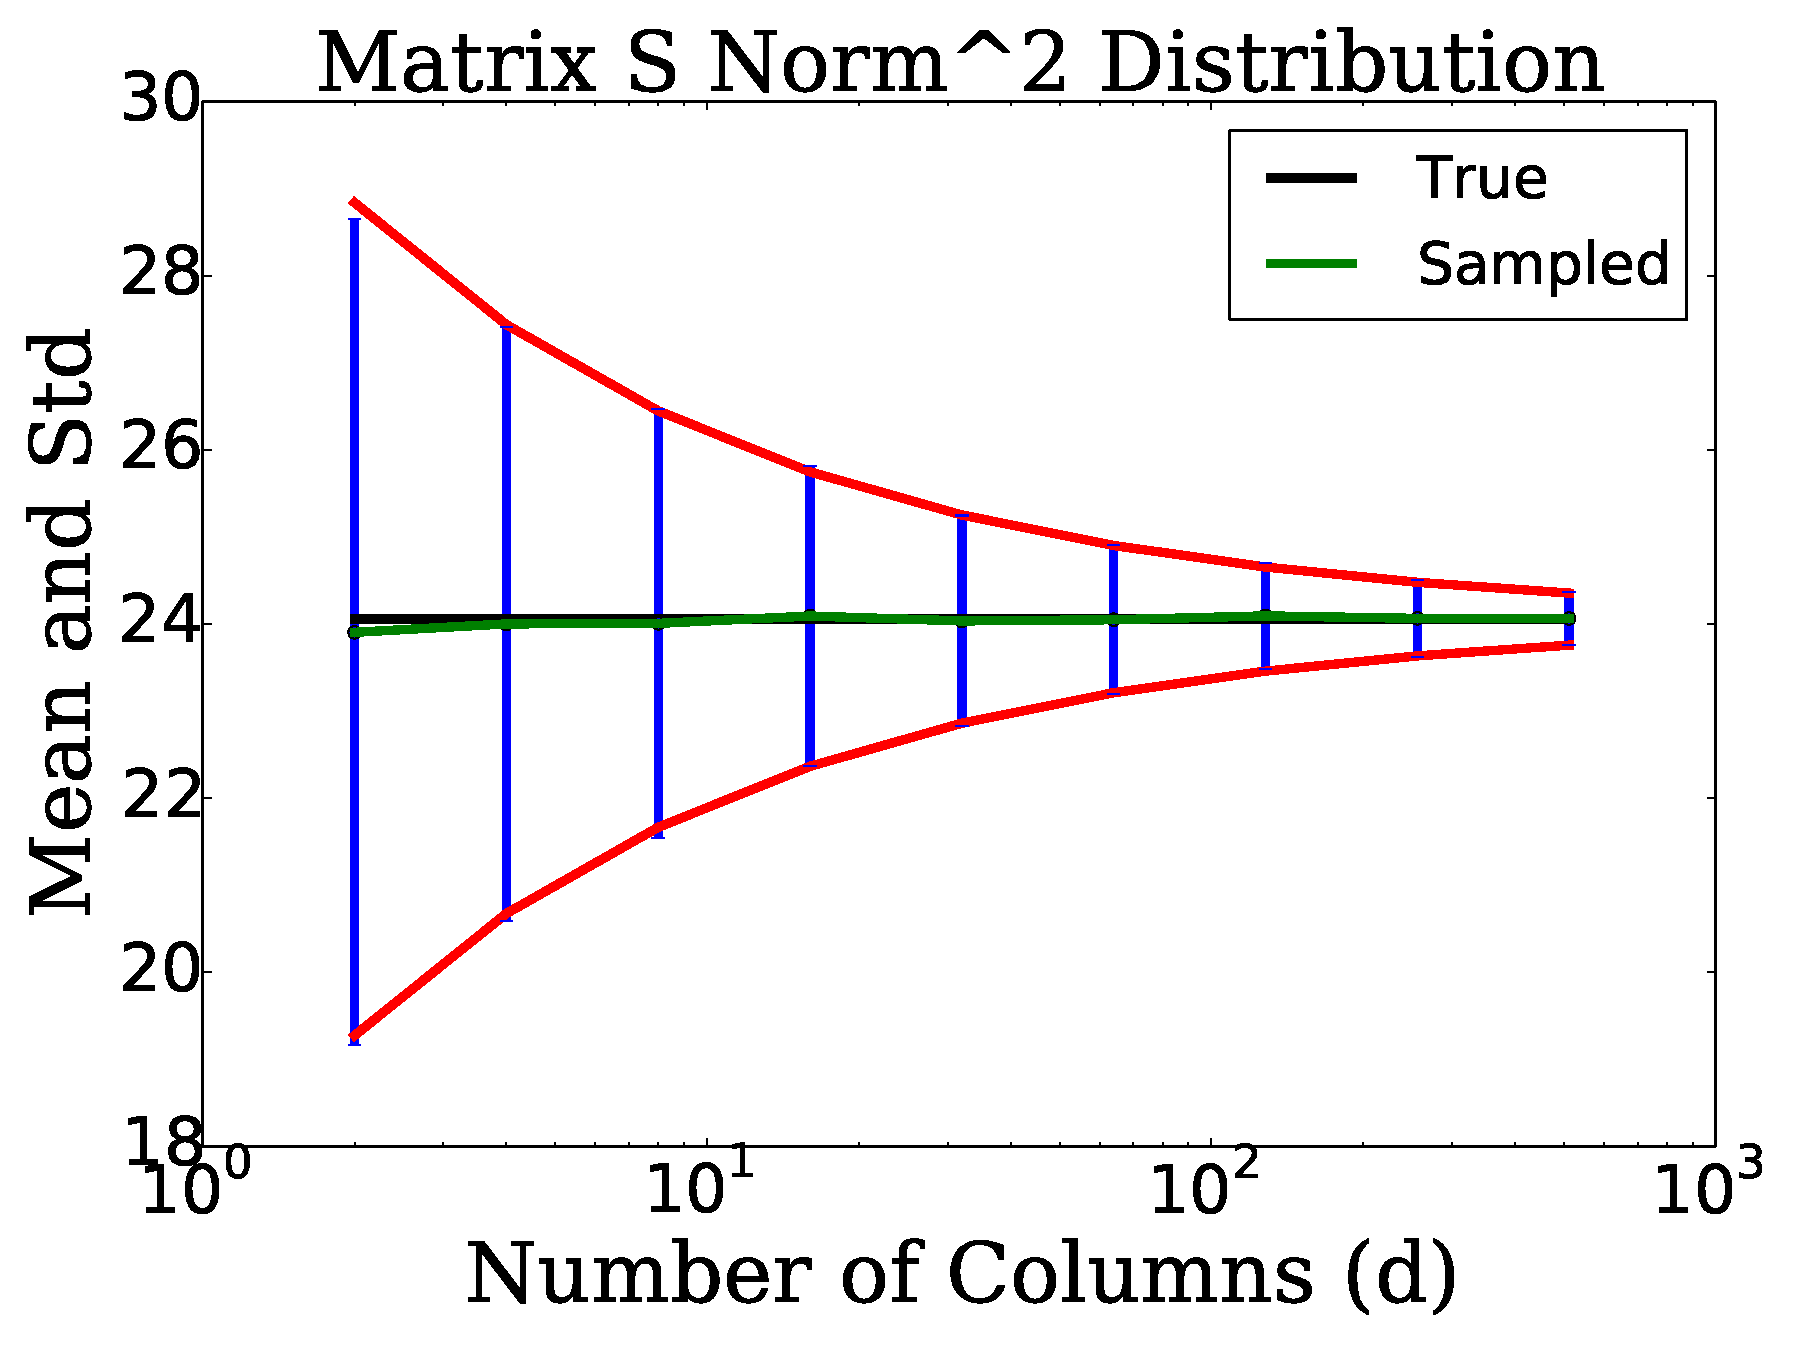
\includegraphics[width=\textwidth]{plots/mat_S_error_test_2.pdf}
    \caption{Matrix S}
    \end{subfigure}
    \begin{subfigure}{0.45\textwidth}
    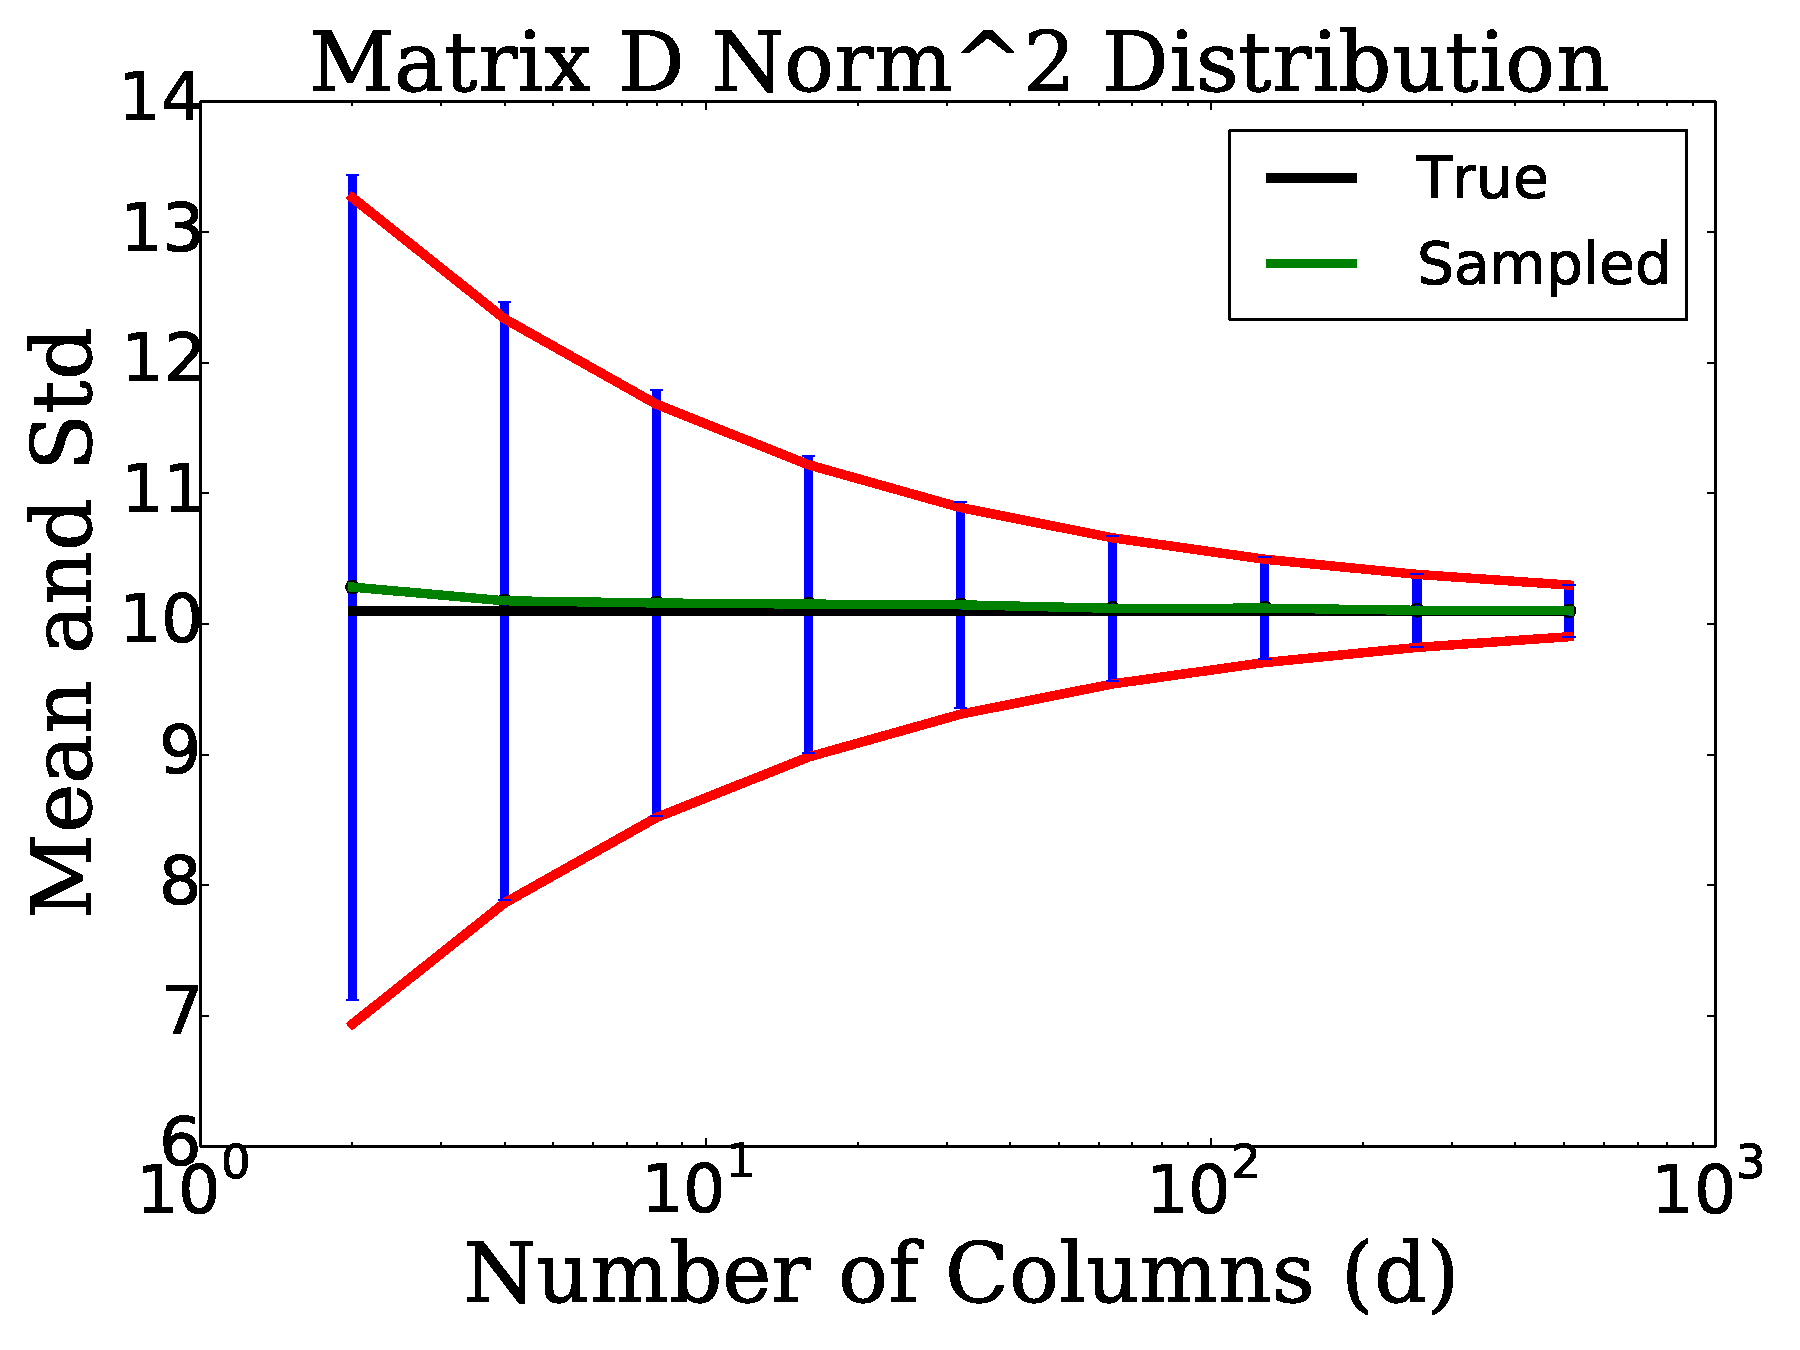
\includegraphics[width=\textwidth]{plots/mat_D_error_test_2.pdf}
    \caption{Matrix D}
    \end{subfigure}

\caption[GEB Stochastic Squared F-norm Approximations]{
%Estimated $||A||_{F}$ for our matrices using the Gaussian Error Bound.
We performed 10,000 trials and computed the
mean (Green) and standard deviation (Blue) of $\norm{A\Omega}_{F}^{2}$
for columns $d\in\{2,4,8,\cdots,512\}$.
The true squared F-norm value is Black and the theoretical standard
deviation bounds from Eq.~\eqref{eq:rand_Xd_variance_bounds} are Red.
}
\label{fig:geb_norm_squared_bound_mat}
\end{figure}






\subsection{Adaptive Comparison}

We now compare some of the adaptive low-rank algorithms;
in particular, we use Alg.~\ref{alg:rand_low_rank} with the HMT
stopping criterion, the YGL algorithm in Alg.~\ref{alg:rand_low_rank_YGL},
and the new randomized low-rank compression algorithm
in Alg.~\ref{alg:rand_new_low_rank}.
Once each algorithm has determined enough random samples have been computed,
a pivoted QR factorization is computed on the entire batch
and the factorization is truncated below the specified tolerance.
This last part (pivoted QR) is not an explicit feature of
Algs.~\ref{alg:rand_low_rank}--\ref{alg:rand_low_rank_YGL} but is added
due to it being necessary in the situation where our new algorithm
was developed~\cite{randomHSSLBL}.
These results can be found in Table~\ref{tab:results_qb_approx_mat};
the minimum samples required to meet the specified tolerance
(as determined by the SVD) are given in Table~\ref{tab:results_qb_min_rank}.
The averaged number of random samples used is computed as well
as the average 2-norm error taken over 1,000 trials.
While the YGL and new algorithm bounds are related to the F-norm,
the 2-norm is of primary importance.
Random samples are computed in blocks of 16 random samples and,
due to the nature of our new algorithm, the minimum possible number of
samples used in Alg.~\ref{alg:rand_new_low_rank} is 32:
16 samples for initial $Q$ and 16 samples for the error estimate.
The YGL algorithm stops if we compute $E\le0$.

From the results, we see that the HMT bound always performs the worst
in every case; this is expected from it overestimating the 2-norm.
Outside of this, the YGL and GEB algorithms are close.
Matrix A1 is particularly challenging: it has slow singular value decay
and our algorithm performs no power iteration.
For this matrix, YGL does better than GEB in every case
(they perform equally well with a relative error of $0.1$), in part
because knowing the error exactly is important.
For Matrix A2, YGL does better for $0.1$ relative error, with GEB
using fewer or equal samples in the other cases.
Matrices E1, E2, and S are similar: YGL and GEB are about the same
for large relative errors but, due to the inherent error bound restrictions,
the new algorithm is better for smaller tolerances.
For Matrix D, YGL did a little better than GEB.
Overall, the results here show that the YGL stopping criterion
may be slightly better than the GEB stopping criterion when
for $\epsr\ge O(\sqrt{\epsm})$, but our stochastic F-norm bound allows us
to determine relative errors to smaller tolerances.

We now perform more runs, except here we only look at the new
stopping criterion;
we set the blocksize to 5 and change the relative tolerances.
Results are shown in Table~\ref{tab:results_qb_approx_mat_geb_hard},
and Table~\ref{tab:results_qb_min_rank_tough_geb} contains the minimum
required ranks.
The relative tolerances here are difficult and are meant to test
the limits of our stopping criterion.
For Matrix E1, we are able to have relative tolerances down to
5E-15 without having any problems with the
stopping criterion (that is, every trial determined 100 samples
was sufficient for the specified tolerance);
some trials failed to satisfy the stopping criterion for 1E-15 and
no trials satisfied the stopping criterion for 5E-16.
These difficulties are expected because we are getting close to
the limitations of machine precision ($\epsm\approx10^{-16}$
for double precision).
For Matrix S, we note that we use an average of 107 samples for
the tolerance 1E-14, which is more than the 100 samples that
should be sufficient ideally.
For Matrix D, we used \textbf{single precision}.
We did not have any problems with relative tolerances down
to 5E-6; for the tolerance 1E-6, most trials (738/1000) failed to
satisfy the stopping criterion.
Again, this is expected because $\epsm\approx10^{-7}$ in single precision.
Overall, we see that our new stopping criterion allows us to get
close to machine precision, which is not the case
when using the HMT or YGL algorithms.

%%%%%%%%%%%%%%%%%%%%%%%%%%%%%%%%%%%%%%%%%%%%%%%%%%%%%%%%%%%%%%%%%%%%%%%%
%%% HMT/YGL/GEB QB Approx table

\begin{table}
\begin{center}
\begin{tabular}{|c|c|c|c|c|c|c|c|c|}
\cline{2-9}
\multicolumn{1}{c|}{} &
\multicolumn{2}{|c|}{\textbf{0.75}} & \multicolumn{2}{|c|}{\textbf{0.5}} &
\multicolumn{2}{|c|}{\textbf{0.25}} & \multicolumn{2}{|c|}{\textbf{0.1}} \\
\hline
Matrix A1 &
Err & Samp & Err & Samp &
Err & Samp & Err & Samp \\
\hline
HMT & 0.19 & 128 & 0.16 & 128 & 0.13 & 128 & 3E-15 & 128 \\
\hline
YGL & 0.45 & 20 & 0.24 & 59 & 0.16 &  96 & 3E-3 & 112 \\
\hline
GEB & 0.22 & 77 & 0.18 & 94 & 0.15 &  102 & 5E-3 & 112 \\
\hline
\hline
\multicolumn{1}{c|}{} &
\multicolumn{2}{|c|}{\textbf{1E-1}} & \multicolumn{2}{|c|}{\textbf{1E-2}} &
\multicolumn{2}{|c|}{\textbf{1E-3}} & \multicolumn{2}{|c|}{\textbf{1E-4}} \\
\hline
Matrix A2 &
Err & Samp & Err & Samp &
Err & Samp & Err & Samp \\
\hline
HMT & 4E-2 & 42 & 3E-3 & 92 & 3E-4 & 128 & 2E-15 & 128 \\
\hline
YGL & 4E-2 & 16 & 5E-3 & 32 & 4E-4 &  96 & 2E-15 & 112 \\
\hline
GEB & 4E-2 & 32 & 5E-3 & 32 & 4E-4 &  80 & 2E-15 & 112 \\
\hline
\hline
\multicolumn{1}{c|}{} &
\multicolumn{2}{|c|}{\textbf{1E-3}} & \multicolumn{2}{|c|}{\textbf{1E-6}} &
\multicolumn{2}{|c|}{\textbf{1E-9}} & \multicolumn{2}{|c|}{\textbf{1E-12}} \\
\hline
Matrix E1 &
Err & Samp & Err & Samp &
Err & Samp & Err & Samp \\
\hline
HMT & 4E-4 & 48 & 4E-7 & 76 & 4E-10 & 96 & 4E-13 & 112 \\
\hline
YGL & 6E-4 & 32 & 7E-7 & 48 & 1E-9  & 64 & 6E-10 & 64 \\
\hline
GEB & 6E-4 & 32 & 7E-7 & 48 & 1E-9  & 65 & 7E-13 & 94 \\
\hline
\hline
\multicolumn{1}{c|}{} &
\multicolumn{2}{|c|}{\textbf{1E-3}} & \multicolumn{2}{|c|}{\textbf{1E-6}} &
\multicolumn{2}{|c|}{\textbf{1E-9}} & \multicolumn{2}{|c|}{\textbf{1E-12}} \\
\hline
Matrix E2 &
Err & Samp & Err & Samp &
Err & Samp & Err & Samp \\
\hline
HMT & 3E-4 & 32 & 3E-7 & 48 & 4E-10 & 53 & 3E-13 & 82* \\
\hline
YGL & 6E-4 & 16 & 4E-7 & 32 & 8E-10 & 32 & 1E-10 & 32 \\
\hline
GEB & 3E-4 & 32 & 4E-7 & 32 & 8E-10 & 32 & 5E-13 & 48 \\
\hline
\hline
\multicolumn{1}{c|}{} &
\multicolumn{2}{|c|}{\textbf{1E-3}} & \multicolumn{2}{|c|}{\textbf{1E-6}} &
\multicolumn{2}{|c|}{\textbf{1E-9}} & \multicolumn{2}{|c|}{\textbf{1E-12}} \\
\hline
Matrix S &
Err & Samp & Err & Samp &
Err & Samp & Err & Samp \\
\hline
HMT & 4E-4 & 64 & 3E-7 & 80 & 4E-10 & 80 & 3E-13 & 200+ \\
\hline
YGL & 5E-4 & 48 & 2E-6 & 48 & 6E-10 & 64 & 2E-11 & 64 \\
\hline
GEB & 5E-4 & 48 & 9E-7 & 59 & 6E-10 & 64 & 6E-13 & 80 \\
\hline
\hline
\multicolumn{1}{c|}{} &
\multicolumn{2}{|c|}{\textbf{1E-1}} & \multicolumn{2}{|c|}{\textbf{1E-3}} &
\multicolumn{2}{|c|}{\textbf{1E-5}} & \multicolumn{2}{|c|}{\textbf{1E-7}} \\
\hline
Matrix D &
Err & Samp & Err & Samp &
Err & Samp & Err & Samp \\
\hline
HMT & 3E-2 & 51 & 4E-4 & 80 & 4E-6 & 96 & 4E-8 & 112 \\
\hline
YGL & 9E-2 & 27 & 6E-4 & 48 & 1E-5 & 64 & 2E-7 & 85 \\
\hline
GEB & 5E-2 & 32 & 6E-4 & 48 & 9E-6 & 69 & 6E-8 & 96 \\
\hline
\end{tabular}
\end{center}
\caption[QB Adaptive Approximation Results]{
QB approximation results for Matrices A1, A2, E1, E2, S, and D.
For each absolute error tolerance, we averaged 1,000 trials to determine
the average error (Err) and average samples used (Samp) in order to compute
a QB approximation once we used either the HMT stopping criterion,
the YGL stopping criterion, or the new stopping criterion to
determine when we had approximated the range.
Random samples were computed in blocks of 16.
In the case when we used $200+$ samples,
we were not able to meet the HMT stopping criterion
and used the maximum of 200 random samples.
Some of the data here was originally in~\cite{randomHSSLBL}.
The minimum possible ranks can be found in Table~\ref{tab:results_qb_min_rank}.
A ``*'' means that there were some runs which reached the maximum allowable
samples of 200 before compression.
}
\label{tab:results_qb_approx_mat}
\end{table}

%%%%%%%%%%%%%%%%%%%%%%%%%%%%%%%%%%%%%%%%%%%%%%%%%%%%%%%%%%%%%%%%%%%%%%%%
%%% HMT/YGL/GEB QB Approx table

\begin{table}
\begin{center}
\begin{tabular}{|c|c|c|c|c|}
\hline
Matrix A1 & \textbf{0.75} & \textbf{0.5} & \textbf{0.25} & \textbf{0.1} \\
\hline
Min Rank  & 1 & 4 & 16 & 100 \\
\hline
\hline
Matrix A2 & \textbf{1E-1} & \textbf{1E-2} & \textbf{1E-3} & \textbf{1E-4} \\
\hline
Min Rank  & 3 & 10 & 31 & 100 \\
\hline
\hline
Matrix E1 & \textbf{1E-3} & \textbf{1E-6} & \textbf{1E-9} & \textbf{1E-12} \\
\hline
Min Rank  & 19 & 38 & 57 & 76 \\
\hline
\hline
Matrix E2 & \textbf{1E-3} & \textbf{1E-6} & \textbf{1E-9} & \textbf{1E-12} \\
\hline
Min Rank  & 9 & 18 & 27 & 36 \\
\hline
\hline
Matrix S  & \textbf{1E-3} & \textbf{1E-6} & \textbf{1E-9} & \textbf{1E-12} \\
\hline
Min Rank  & 35 & 45 & 55 & 65 \\
\hline
\hline
Matrix D  & \textbf{1E-1} & \textbf{1E-3} & \textbf{1E-5} & \textbf{1E-7} \\
\hline
Min Rank  & 20 & 40 & 60 & 80 \\
\hline
\hline
\end{tabular}
\end{center}
\caption[QB Adaptive Test: Minimum Rank]{
Here are the absolute minimum ranks required
for Matrices A1, A2, E1, E2, S, and D.
}
\label{tab:results_qb_min_rank}
\end{table}


%%%%%%%%%%%%%%%%%%%%%%%%%%%%%%%%%%%%%%%%%%%%%%%%%%%%%%%%%%%%%%%%%%%%%%%%
%%% HMT/YGL/GEB QB Approx table

\begin{table}
\begin{center}
\begin{tabular}{|c|c|c|c|c|c|c|c|c|}
\cline{2-9}
\multicolumn{1}{c|}{} &
\multicolumn{2}{|c|}{\textbf{1E-14}} & \multicolumn{2}{|c|}{\textbf{5E-15}} &
\multicolumn{2}{|c|}{\textbf{1E-15}} & \multicolumn{2}{|c|}{\textbf{5E-16}} \\
\hline
Matrix E1 &
Err & Samp & Err & Samp &
Err & Samp & Err & Samp \\
\hline
GEB & 1E-14 & 97 & 4E-15 & 100 & 6E-16  & 144* & 7E-16 & 200+ \\
\hline
\hline
\multicolumn{1}{c|}{} &
\multicolumn{2}{|c|}{\textbf{5E-13}} & \multicolumn{2}{|c|}{\textbf{1E-13}} &
\multicolumn{2}{|c|}{\textbf{4E-14}} & \multicolumn{2}{|c|}{\textbf{1E-14}} \\
\hline
Matrix S &
Err & Samp & Err & Samp &
Err & Samp & Err & Samp \\
\hline
GEB & 4E-13 & 75 & 7E-14 & 96 & 5E-14 & 100 & 9E-15 & 107 \\
\hline
\hline
\multicolumn{1}{c|}{} &
\multicolumn{2}{|c|}{\textbf{5E-5}} & \multicolumn{2}{|c|}{\textbf{1E-5}} &
\multicolumn{2}{|c|}{\textbf{5E-6}} & \multicolumn{2}{|c|}{\textbf{1E-6}} \\
\hline
Matrix D &
Err & Samp & Err & Samp &
Err & Samp & Err & Samp \\
\hline
GEB (s) & 4E-5 & 59 & 9E-6 & 66 & 9E-6 & 71 & 6E-7 & 186* \\
\hline
\end{tabular}
\end{center}
\caption[QB Adaptive Approximation Results (Stringent GEB Tests)]{
Tough QB approximation results for Matrices E1, S, and D
using the new GEB stopping criterion.
For each absolute error tolerance, we averaged 1,000 trials to determine
the average error (Err) and average samples used (Samp) in order to compute
a QB approximation once we used the new stopping criterion to
determine when we had approximated the range.
Random samples were computed in blocks of 5.
For matrix D, we used \textbf{single precision}.
In the case when we used $200+$ samples,
we were not able to meet the HMT stopping criterion
and used the maximum of 200 random samples.
The minimum possible ranks can be found in
Table~\ref{tab:results_qb_min_rank_tough_geb}.
A ``*'' means that there were some runs which reached the maximum allowable
samples of 200 before compression.
For matrix E1 with $\epsr$=1E-15, 7.7\% of the trials used over 200 samples
(and so failed to stop);
for matrix D  with $\epsr$=1F-6, 73.8\% of the trials used over 200 samples.
}
\label{tab:results_qb_approx_mat_geb_hard}
\end{table}

%%%%%%%%%%%%%%%%%%%%%%%%%%%%%%%%%%%%%%%%%%%%%%%%%%%%%%%%%%%%%%%%%%%%%%%%
%%% HMT/YGL/GEB QB Approx table

\begin{table}
\begin{center}
\begin{tabular}{|c|c|c|c|c|}
\hline
Matrix E1 & \textbf{1E-14} & \textbf{5E-15} & \textbf{1E-15} & \textbf{5E-16} \\
\hline
Min Rank  & 88 & 90 & 95 & 96 \\
\hline
\hline
Matrix S  & \textbf{5E-13} & \textbf{1E-13} & \textbf{5E-14} & \textbf{1E-14} \\
\hline
Min Rank  & 66 & 69 & 71 & 100 \\
\hline
\hline
Matrix D  & \textbf{5E-5} & \textbf{1E-5} & \textbf{5E-6} & \textbf{1E-6} \\
\hline
Min Rank  & 50 & 60 & 60 & 70 \\
\hline
\hline
\end{tabular}
\end{center}
\caption[QB Adaptive Test: Minimum Rank (Stringent GEB Test)]{
Here are the absolute minimum ranks required for Matrices E1, S, and D.
}
\label{tab:results_qb_min_rank_tough_geb}
\end{table}




\subsection{Stopping Criteria Discussion}

The results of this section show our new stopping criterion does well,
usually being on par or better than other stopping criteria
while allowing for small tolerances.
One noticeable difficultly, shared by others, is using too many
additional samples to perform a low-order approximation
($\epsr\gtrsim0.1$) for matrices with slow decay without using power iteration;
part of the difficulty comes from using F-norm
bounds when desiring 2-norm accuracy.
Outside of this limited range, the error closely matches
the specified tolerance, keeping communication-heavy computations
to one rank-revealing QR factorization.
Additionally, we showed our stopping criterion
allows us to approximate matrices to relative tolerances
close to machine precision.

